\chapter{Elliptic Curves}
TODO: Elliptic Curve asymmetric cryptography examples. Private key, generator, public key. 
%references http://infosec.pusan.ac.kr/wp-content/uploads/2019/09/Pairings-For-Beginners.pdf
Generally speaking, elliptic curves are "curves" defined in geometric planes like the Euklidean or the projective plane over some given field. One of the key features of elliptic curves over finite fields from the point of view of cryptography is their set of points has a group law, such that the resulting group is finite and cyclic and it is believed that the discrete logarithm problem on these groups is hard. 

A special class of elliptic curves are so called \textit{pairing friendly curve}, which have a notation of a group pairing as defined in XXX. This pairing has cryptographicall nice prperties. Those curve are useful in the development of SNAKS, since they allow to compute so called R1CS-satisfiability "in the exponent" (THIS HAS TO BE REWRITTEN WITH WAY MORE DETAIL)

In this chapter we introduce epileptic curves as they are used in pairing based approaches to the construction of snarks. The eliptic curves we consider are all defined over prime fields or prime field extensions and the reader should be familiar with the contend of the previous section on those fields.

In its most generality elliptic curves are defined as a smooth projective curve of genus 1 defined over some field $\F$ with a distinguished $\F$-rational point, but this definition is not very useful for the introductary character of this book. We will therefore look at $3$ more practical definitions in the following sections, by introducing Weierstraß, Montgommery and Edwards curves. All of them are useful in cryptography and nesessary to understand for the contnuation of the book.

\section{Elliptic Curve Arithmetics}

\subsection{Short Weierstraß Curves}
In this section we introduce the so called short Weierstraß curves, which are the most general types of curves over finite fields of characteristic greater then $3$. 

We start with their reprrsention in affine space. This reprresentation has the advantage that affine points are just pairs of numbers which is more convinient to work with for the beginner. However it has the disadvantage that a special "point at infinity" that is not a point on the curve, is necessary to describe the group structure. We introduce the elliptic curve group law and describe elliptic curve scalar multiplication, which is nothing but an instatation of the exponential map from general cyclic groups.

Then we look at the projective representation of short Weierstrass curves. It has the advantage that no special sybol is necessary to represent the point at infinity but comew with the drawback that projective points are classes of numbers, which might be a bit unusual for a beginner.

We finish this section with an explicit equivalence that transforms affine representations into projective once and vice versa.

\paragraph{Affine short Weierstraß form} Probably the least abstract and most straight forward way to introduce elliptic curves for non-mathematicians and beginners is the so called affine representation of a short Weierstraß curve. To see what this is, let $\F$ be a finite field of order $q$ and $a,b\in \F$ two field elements such that $\Zmod{4a^3+ 27b^2}{q}\neq 0$. Then a \textbf{short Weierstrass elliptic curve} $E(\F)$ over $\F$ in its affine representation is the set
\begin{equation}
\label{def_short_weierstrass_curve}
E(\F) = \{(x,y)\in \F\times \F\;|\; y^2=x^3+a\cdot x+b \} \bigcup \{\Oinf\}
\end{equation}
of all pairs of field elements $(x,y)\in \F\times \F$, that satisfy the short Weierstrass cubic equation $y^2=x^3+a\cdot x+b$, together with a distingushid symbol $\Oinf$, called the \textbf{point at infinity}.
\begin{notation}
In the literature, the set $E(\F)$, which includs the sybol $\mathcal{O}$ is often called the set of \textit{rational points} of the elliptic curve, in which case the curve itself is usually written as $E/\F$. However in what follows we will frequently identify an elliptic curve with its set of rational points and therefore use the symbol $E(\F)$ instead. This is possible in our case, since we only really care about the group structure of the curve in consideration.
\end{notation}
The term "curve" appears, because in the ordinary 2 dimensional plane $\R^2$,
the set of all points $(x,y)$ that satisfy $y^2 = x^3 +a\cdot x +b$ looks like a curve. We should note however, that visualizing elliptic curves over finite fields as "curves" has its limitations and we will therefore not stress the geometric picture too much, but focus on the compuational properties instead. To understand the visual difference, consider the following two elliptic curves: 
% let sage draw some elliptic curve in R^2, but show only the picture
\begin{sagesilent}
E1 = EllipticCurve([-2,1])
C1 = E1.plot()
F = GF(9973)
E2 = EllipticCurve(F, [-2,1])
C2 = E2.plot()
\end{sagesilent}
\begin{center} 
\sageplot[scale=.5]{C1} 
\sageplot[scale=.5]{C2}
\end{center}
% TODO: PLOT BOTH CURVES ON THE SAME LINE NOT BELOW EACH OTHER
Both elliptic curves are defined by the same short Weierstraß equation $y^2 = x^3-2x+1$, but the first curve is define in the real affine plane $\mathbb{R}^2$, that is the pair $(x,y)$ contains real numbers, while the second one is defined in the affine plane $\F_{9973}^2$, which means that both $x$ and $y$ are from the prime field $\F_{9973}$. Every blue dot represents a pair $(x,y)$ that is solution to $y^2 = x^3-2x+1$ and as we can see the second curve hardly looks like a geometric structure one would naturally call a curve. So the geometric intuitions from $\R^2$ is kind of obfuscated in curves over finite fields.

The identity $\Zmod{6\cdot(4a^3+ 27b^2)}{q}\neq 0$ ensures that the curve is  non-singular, which basically means that the curve has no cusps or self-intersections.

When dealing with elliptic curves compuations can quickly become cumbersome and tedious. So on the one hand side the reader is adviced to do as many compuations in a pen and paper style as possible. This helps a lot to get a deeper understanding for the details. On the other hand side however, compuations are sometimes simply to large to be done by hand and one might get lost in the details. Fortunately sage is very helpful in dealing with elliptic curves. It is there a goal of this book to introduce the reader to the great elliptic curve capabilities of sage. One we to define elliptic curves and work is them goes like this:
\begin{sagecommandline}
sage: F5 = GF(5) # define the base field
sage: a = F5(2) # parameter a
sage: b = F5(4) # parameter b
sage: # check non-sigularity
sage: F5(6)*(F5(4)*a^3+F5(27)*b^2) != F5(0)
sage: # short Weierstrass curve 
sage: E = EllipticCurve(F5,[a,b]) # y^2 == x^3 + ax +b 
sage: P = E(0,2) # 2^2 == 0^3 + 2*0 + 4
sage: P.xy() # affine coordinates
sage: INF = E(0) # point at infinity
sage: try: 	# point at infinity has no affine coordinates
....:     INF.xy()
....: except ZeroDivisionError:
....:     pass
sage: P = E.plot() # create a plotted version 
\end{sagecommandline}
The following three examples will give a more practical understanding of what an elliptic curve is and how we can compute them. The reader is adviced to read them carefully and ideally to parallel the computation themselfs. We will repeatedly build on these example in this chapter and use the second example at various places in this book.
\begin{example}To provide the reader with a small example of an elliptic curve, where all computation can e done in a pen and paper style, consider the prime field $\F_5$ from example (XXX). The reader who had worked through the examples and exercises in the previous section knows this prime field well.

To define an elliptic curve over $\F_5$, we have to choose to numbers $a$ and $b$ from that field. Assuming we choose $a=1$ and $b=1$ then $\kongru{4a^3+ 27b^2}{1}{5}$ from which follows that the corresponding elliptic curve $E_1(\F_5)$ is given by the set of all pairs $(x,y)$ from $\F_5$ that satisfy the equation $y^2=x^3+x+1$, together with the special symbol $\Oinf$, which represents the "point at infinity". 

To get a better understand of that curve, obersever that if we choose arbitrarily the pair $(x,y)=(1,1)$, we see that $1^2 \neq 1^3+1 + 1$ and hence $(1,1)$ is not an element of the curve $E_1(\F_5)$. On the other hand chosing for exmple $(x,y)=(2,1)$ gives $1^2 = 2^3 + 2 + 1$ and hence the pair $(2,1)$ is an element of $E_1(\F_5)$ (Remember that all computations are done in modulo $5$ arithmetics).

Now since the set $\F_5\times \F_5$ of all pairs $(x,y)$ from $\F_5$ contains only $5\cdot 5=25$ pairs, we can compute the curve, by just inserting every possible pair $(x,y)$ into the short Weierstraß equation $y^2 = x^3 + x +1$. If the equation holds, the pair is a curve point, if not that means that the point is not on the curve. Combining the result of this computation with the point at infinity gives the curve as:
$$
E_1(\F_5) = \{\Oinf, (0,1),(2,1),(3,1),(4,2),(4,3),(0,4),(2,4),(3,4)\}
$$
So our elliptic curve is a set of $9$ elements. $8$ of which are pairs of numbers and one special symbol $\Oinf$. Visualizing $E1$ gives:
\begin{sagesilent}
F5 = GF(5)
E1 = EllipticCurve(F5, [1,1])
C1 = E1.plot()
\end{sagesilent}
\begin{center} 
\sageplot[scale=.5]{C1}
\end{center}
% sage: AffinePoints = [P.xy() for P in E1.points() if P.order > 1]
\end{example}
In the development of SNARKS it is sometimes necessary to do elliptic curve cryptograph "in a circuit", which basically means that the elliptic curves needs to be implemented in a certain SNARK-friedly way. We will look at what this means in XXX. To be able to do this efficiently it is desireable to have curves with special properties. The following example is a pen and paper version of such a curve, that parallels the definition of a cryptographically secure curve called \textit{Baby-JubJub} which is extensively used in real world snarks. The interested reader is adviced to read this example carefully as we will use it and build on it in various places throughout the book.
\begin{example}[Pen-JubJub] Consider the prime field $\F_{13}$ from exercise XXX. If we choose $a=8$ and $b=8$ then $\kongru{4a^3+ 27b^2}{6}{13}$ and the corresponding elliptic curve is given by all pairs $(x,y)$ from $\F_13$ such that $y^2=x^3+8x+8$ holds. We write $\mathit{PJJ\_13}$ for this curve and call it the \textit{Pen-JubJub} curve.

Now since the set $\F_{13}\times \F_{13}$ of all pairs $(x,y)$ from $\F_{13}$ contains only $13\cdot 13=169$ pairs, we can compute the curve, by just inserting every possible pair $(x,y)$ into the short Weierstraß equation $y^2 = x^3 +8x +8$.  We get 
\begin{multline*}
\mathit{PJJ\_13} = \{\Oinf, (1, 2), (1, 11), (4, 0), (5, 2), (5, 11), (6, 5), (6, 8), (7,2), (7, 11), \\ (8, 5), (8, 8), (9, 4), (9, 9), (10, 3), (10,
10), (11, 6), (11, 7), (12, 5), (12, 8)\}
\end{multline*}
As we can see the curve consist of $20$ points. $19$ points from the affine plane and the point at infinity.
To get a visual impression of the $\mathit{PJJ\_13}$ curve, we might plot all of its points (except the point at infinity) in the $\F_{13}\times \F_{13}$ affine plane. We get: 
\begin{sagesilent}
F13 = GF(13)
PJJ_13 = EllipticCurve(F13, [8,8])
CPJJ_13 = PJJ_13.plot()
\end{sagesilent}
\begin{center} 
\sageplot[scale=.5]{CPJJ_13}
\end{center}
As we will see in what follows this curve is kind of special as it is possible to represent it in two alternitive forms, called the Montgomery and the twisted Edwards form (See xxx and XXX).
\end{example}
Now that we have seen two pen and paper friendly elliptic curves, lets look at a curve that is used in actual cryptography. Cryptographically secure elliptic curve are not qualitatively defferent from the curves we looked at so far. The only difference is that the prime number modulus of the prime field is much larger. Typical examples use prime numbers, which have binary representations in the size of more then double the size of the desired security level. So if for example a security of $128$ bit is desired, a prime moduls of binary size $\geq 256$ is choosen. The following example provides such a curve. 
\begin{example}[Bitcoin's Secp256k1 curve]To give an example of a real world, cryptographically secure curve, lets look at curve Secp256k1, which is famous for being used in the public key cryptography of Bitcoin. The prime field $\F_p$ of Secp256k1 if defined by the prime number
$$
p = \scriptstyle 115792089237316195423570985008687907853269984665640564039457584007908834671663
$$
which has a binary representation that need $256$ bits. This implies that the $\F_p$ approximately contains $2^{256}$ many elements. So the underlying field is large. To get an image of how large the base field is, consider that the number $2^{256}$ is approximately in the same order of magnitute as the estimated number of atomes in the observeable universe. 

Curve Secp256k1 is then defined by the parameters $a,b\in \F_p$ with $a=0$ and $b=7$. Since $\Zmod{4\cdot 0^3 + 27\cdot 7^2}{p}=1323$, those parameters indeed define an elliptic curve given by
$$
\mathit{Secp256k1} = \{(x,y)\in \F_p\times \F_p\;| y^2 = x^3 +7\;\} 
$$
Clearly Secp256k1 is a curve, to large to do computations by hand, since it can be shown that $\mathit{Secp256k1}$ contains 
$$
r = \scriptstyle 11579208923731619542357098500868790785283756427907490438260516
3141518161494337
$$
many elements, were $r$ is a prime number that also has a binary representation of $256$ bits. Cryptographically secure elliptic curves are therefore not useful in pen and paper computations. Fortunately sage handles large curve efficiently:
\begin{sagecommandline}
sage: p = 115792089237316195423570985008687907853269984665640564039457584007908834671663
sage: # Hexadecimal representation
sage: p.str(16)
sage: p.is_prime()
sage: p.nbits()
sage: Fp = GF(p)
sage: Secp256k1 = EllipticCurve(Fp,[0,7])
sage: r = Secp256k1.order() # number of elements
sage: r.str(16)
sage: r.is_prime()
sage: r.nbits()
\end{sagecommandline}
%\seqsplit{115792089237316195423570985008687907853269984665640564039457584007908834671663}
\end{example}
\begin{exercise}
Look-up the definition of curve BLS12-381, implement it in sage and computes its order.
\end{exercise}
\paragraph{Affine compressed representation} As we have seen in example XXX, cryptographically secure elliptic curves are definec over large prime fields, where elements of those fields typically need more then $255$ bits storage on a computer. Since elliptic curve points consists of pairs of those field element, they need double that amount of storage.

To reduce the amount of space needed to represent a curve point note however, that up to a sign the $y$-coordinate of a curve point can be computed from the $x$-coordinate, by simply inserting $x$ into the Weierstraß equation and then computing the roots of the result. This gives two results and it follows that we can represent a curve point in \textbf{compressed form} by simply storing the $x$-coordinate together with a single sign bit only, the latter of which deterministically decides which of the two roots to choose. In case that the $y$-coordinate is zero, both sign bit give the same result.

For example one convention could be to always choose the root closer to $0$, when the sign bit is $0$ and the root closer to the order of $\F$ when the sign bit is $1$.

\begin{example}[Pen-JubJub] To understand the concept of compressed curve points a bit better consider the $\mathit{PJJ\_13}$ curve from example XXX again. Since this curve is defined over the prime field $\F_{13}$ and numbers between $0$ and $13$ need approximately $4$ bits to be represented, each $\mathit{PJJ\_13}$ -point need $8$-bits of storage in uncompressed form, while it would need only $5$ bits in compressed form. To see how this works, recall that in uncompressed form we have
\begin{multline*}
\mathit{PJJ\_13} = \{\Oinf, (1, 2), (1, 11), (4, 0), (5, 2), (5, 11), (6, 5), (6, 8), (7,2), (7, 11), \\ (8, 5), (8, 8), (9, 4), (9, 9), (10, 3), (10,
10), (11, 6), (11, 7), (12, 5), (12, 8)\}
\end{multline*}
Using the technique of point compression, we can replace the $y$-ccordinate in each $(x,y)$ pair by a sign bit, indicating, wheather or not $y$ is closer to $0$ or to $13$. So $y$ values in the range $[0,\ldots,6]$ having sign bit $0$ and $y$-values in the range $[7,\ldots,12]$ having sign bit $1$. Applying this to the points in $\mathit{PJJ\_13}$ gives the compressed representation:
\begin{multline*}
\mathit{PJJ\_13} = \{\Oinf, (1, 0), (1, 1), (4, 0), (5, 0), (5, 1), (6, 0), (6, 1), (7,0), (7, 1), \\ (8, 0), (8, 1), (9, 0), (9, 1), (10, 0), (10,1), (11, 0), (11, 1), (12, 0), (12, 1)\}
\end{multline*} 
Note that the numbers $7,\ldots, 12$ are the negatives (additive inverses) of the numbers $1,\ldots, 6$ in modular $13$ arithmetics and that $-0=0$. Calling the compression bit a "sign bit" therefore makes sense.

To recover the uncompressed point of say $(5,1)$, we insert the $x$-ccordinate $5$ into the Weierstraß equation and get $y^2 = 5^3 + 8\cdot 5 +8 = 4$. As expected $4$ is a quadratic residue in $\F_{13}$ with roots $\sqrt{4}= \{2,11\}$. Now since the sign bit of the point is $1$, we have to choose the root closer to the modulus $13$ which is $11$. The uncompressed point is therefore $(5,11)$. 
\end{example}
Looking at the previous examples, compression rate looks not very impressive. The followin example therefore looks at the Secp256k1 curve to show that compression is actually useful.
\begin{example}
Consider the Secp256k1 curve from example XXX again. The following code involves sage to generate a random affine curve point, we then apply our compression method   
\begin{sagecommandline}
sage: P = Secp256k1.random_point().xy()
sage: P
sage: # uncompressed affine point size
sage: ZZ(P[0]).nbits()+ZZ(P[1]).nbits()
sage: # compute the compression
sage: if P[1] > Fp(-1)/Fp(2):
....:     PARITY = 1
....: else:
....:     PARITY = 0
sage: PCOMPRESSED = [P[0],PARITY]
sage: PCOMPRESSED
sage: # compressed affine point size
sage: ZZ(PCOMPRESSED[0]).nbits()+ZZ(PCOMPRESSED[1]).nbits()
\end{sagecommandline}
\end{example}
\paragraph{Affine group law}
%group law
% http://wwwmayr.informatik.tu-muenchen.de/konferenzen/Jass07/courses/1/Lukyanenko/Lukyanenk_Paper.pdf
One of the key properties of an elliptic curve is that it is possible to define a group law on the set of its rational points, such that the point at infinity serves as the neutral element and inverses are reflections on the $x$-axis.

The origin of this law can be understood in a geometric picture and is known as the \textit{chord-and-tangent rule}. In the affine representation of a short Weierstraß curve, the rule can be described in the following way:
\begin{itemize}
\item (Point addition) Let $P, Q\in E(\F)\textbackslash \{\Oinf\}$ with $P\neq Q$ be two distinct points on an elliptic curve, that are both not the point at infinity. Then the sum of $P$ and $Q$ is defined as follows: Consider the line $l$ which intersects the curve in $P$ and $Q$. If $l$ intersects the elliptic curve at a third point $R'$, define the sum $R=P+Q$ of $P$ and $Q$ as the reflection of $R'$ at the $x$-axis. If it does not intersect the curve at a third point define the sum to be the point at infinity $\Oinf$. It can be shown, that no such chord-line will intersect the curve in more then three points, so addition is not ambigious.
\item (Point doubling) Let $P \in E(\F)\textbackslash \{\Oinf\}$ be a point on an elliptic curve, that is not the point at infinity. Then the sum of $P$ with itself (the doubling) is defined as follows: Consider the line wich is tangent to the elliptic curve at $P$, if this line intersects the elliptic curve at a second point $R'$. The sum $2P=P+P$ is then the reflection of $R'$ at the $x$-axis. If it does not intersect the curve at a third point define the sum to be the point at infinity $\Oinf$. It can be shown, It can be shown, that no such tangent-line will intersect the curve in more then two points, so addition is not ambigious.
\item (Point at infinity) We define the point at infinity $\Oinf$ as the neutral ement of addition, that is we define $P+\Oinf = P$ for all points $P\in E(\F)$.
\end{itemize}
It can be shown that the points of an elliptic curve form a commutative group with respect to the tangent and chord rule, such that $\Oinf$ acts the neutral element and the inverse of any element $P\in E(\F)$ is the reflection of $P$ on the $x$-axis.

To translate the geometric description into algebraic equations, first observe that for any two given curve points $(x_1,y_1), (x_2,y_2)\in E(\F)$, it can be shown that the identity $x_1=x_2$ implies $y_2=\pm y_1$, which shows that the following rules are a complete description of the affine addition law.
\begin{itemize}
\item (Neutral element) Point at infinity $\Oinf$ is the neutral element.
\item (Additive inverse ) The addivive inverse of $\mathcal{O}$ is $\mathcal{O}$ and for any other curve point $(x,y) \in E(\F)\textbackslash \{\mathcal{O}\}$, the additive inverse is given by $(x,-y)$.
\item (Addition rule) For any two curve points $P, Q \in E(\F)$ addition is defined by one of the following three cases:
\begin{enumerate}
\item (Adding the neutral element) If $Q=\Oinf$, then the sum is defined as $P+Q=P$.
\item (Adding inverse elements)  If $P=(x,y)$ and $Q=(x,-y)$, the sum is defined as $P+Q=\Oinf$.
\item (Adding non self-inverse equal points) If $P=(x,y)$ and $Q=(x,y)$ with $y\neq 0$, the sum $2P=(x',y')$ is defined by
$$
\begin{array}{llr}
x' = \left(\frac{3x^2+a}{2y}\right)^2 -2x &,&
y' = \left(\frac{3x^2+a}{2y}\right)^2\left(x-x'\right) - y
\end{array} 
$$
\item (Adding non inverse differen points) If $P=(x_1,y_1)$ and $Q=(x_2,y_2)$ such that $x_1 \neq x_2$, the sum $R=P+Q$ with $R=(x_3,y_3)$ is defined by
$$
\begin{array}{llr}
x_3 = \left(\frac{y_2-y_1}{x_2-x_1}\right)^2 -x_1-x_2 &, &
y_3 = \left(\frac{y_2-y_1}{x_2-x_1} \right)\left(x_1-x_3\right) - y_1
\end{array} 
$$
\end{enumerate}
 
\end{itemize} 
Note that short Weierstraß curve points $P$ with $P=(x,0)$ are inverse to themselfs, which implies $2P=\Oinf$ in this case.

As we can see, it is very efficient to compute inverses on elliptic curves. However computing the addition of elliptic curve points in the affine representation needs to consider many cases and involves extensive finite field divisions. As we will see in the next paragraph this can be simplified in projective coordinates.

To get some practical impression of how the group law on an elliptic curve is computed, lets look at some actual cases: 
\begin{example}Consider the elliptic curve $E_1(\F_5)$ from example XXX again.  As we have seen, the set of rational points contains $9$ elements and is given by
$$
E_1(\F_5) = \{\Oinf, (0,1),(2,1),(3,1),(4,2),(4,3),(0,4),(2,4),(3,4)\}
$$
We know that this set defines a group, so we can add any two elements from $E_1(\F_5)$ to get a third element. 

To give an example consider the elements $(0,1)$ and $(4,2)$. Neither of these elements is the neutral element $\Oinf$ and since the $x$-coordinate of $(0,1)$ is different from the $x$-coordinate of $(4,2)$, we know that we have to use the chord rule, that is rule number 4 from XXX to compute the sum $(0,1)\oplus (4,2)$. We get
%\begin{tabular}{lr}
\begin{align*}
x_3  & = \left(\frac{y_2-y_1}{x_2-x_1}\right)^2 -x_1-x_2 & \text{\# insert points}\\
     & = \left(\frac{2-1}{4-0}\right)^2 -0-4  & \text{\# simplify in } \F_5\\
     & = \left(\frac{1}{4}\right)^2 +1
       = 4^2 +1
       = 1 +1 
       = 2
\\
\\
y_3  & = \left(\frac{y_2-y_1}{x_2-x_1} \right)\left(x_1-x_3\right) - y_1  & \text{\# insert points}\\     
     & = \left(\frac{2-1}{4-1} \right)\left(0-2\right) - 1   & \text{\# simplify in } \F_5\\    
     & = \left(\frac{1}{4} \right)\cdot 3 + 4   
       = 4\cdot 3 + 4
       = 2 + 4
       = 1          
\end{align*} 
%\end{tabular}
So in our elliptic curve $E_1(\F_5)$ we get $(0,1)\oplus (4,2) =(2,1)$ and indeed the pair $(2,1)$ is an element of $E_1(\F_5)$ as expected. On the other hand we have $(0,1)\oplus (0,4) =\Oinf$, since both points have equal $x$-coordinates and inverse $y$-coordinates rendering them as inverse to each other. Adding the point $(4,2)$ to itself, we have to use the tangent rule, that is rule 3 from XXX. We get 
\begin{align*}
x'  & = \left(\frac{3x^2+a}{2y}\right)^2 -2x   & \text{\# insert points}\\
    & = \left(\frac{3\cdot 4^2+1}{2\cdot 2}\right)^2 -2\cdot 4 & \text{\# simplify in } \F_5 \\
    & = \left(\frac{3\cdot 1+1}{4}\right)^2 +3\cdot 4
      = \left(\frac{4}{4}\right)^2 +2
      = 1 +2 
      = 3
\\
\\
y'  & = \left(\frac{3x^2+a}{2y}\right)^2\left(x-x'\right) - y  & \text{\# insert points} \\
    & = \left(\frac{3\cdot 4^2+1}{2\cdot 2}\right)^2\left(4-3\right) - 2 & \text{\# simplify in } \F_5\\
    & = 1\cdot 1 + 3
      = 4
\end{align*}
So in our elliptic curve $E_1(\F_5)$ we get the doubling $2\cdot (4,2)$, that is $(4,2)\oplus (4,2) =(3,4)$ and indeed the pair $(3,4)$ is an element of $E_1(\F_5)$ as expected. The group $E_1(\F_5)$ has no self inverse points other then the neutral element $\Oinf$, since no point has $0$ as its $y$-coordinate. We can invoke sage to double check the computations. 
\begin{sagecommandline}
sage: F5 = GF(5)
sage: E1 = EllipticCurve(F5,[1,1])
sage: INF = E1(0) # point at infinity
sage: P1 = E1(0,1)
sage: P2 = E1(4,2)
sage: P3 = E1(0,4)
sage: R1 = E1(2,1)
sage: R2 = E1(3,4)
sage: R1 == P1+P2
sage: INF == P1+P3
sage: R2 == P2+P2
sage: R2 == 2*P2
sage: P3 == P3 + INF
\end{sagecommandline}
\end{example}
\begin{example}[Pen-JubJub] Consider the $\mathit{PJJ\_13}$-curve from example XXX again and recall that its group of rational points is given by 
\begin{multline*}
\mathit{PJJ\_13} = \{\Oinf, (1, 2), (1, 11), (4, 0), (5, 2), (5, 11), (6, 5), (6, 8), (7,2), (7, 11), \\ (8, 5), (8, 8), (9, 4), (9, 9), (10, 3), (10,
10), (11, 6), (11, 7), (12, 5), (12, 8)\}
\end{multline*}
In contrast to the group from the previous example, this group contains a self inverse point, which is different from the neutral element, given by $(4,0)$. To see what this means, observe that we can not add $(4,0)$ to itself using the tangent rule 3 from XXX, as the $y$-coordinate is zero. Instead we have to use rule 2, since $0=-0$. We therefore get $(4,0)\oplus (4,0)=\Oinf$ in $\mathit{PJJ\_13}$. The point $(4,0)$ is therefore inverse to itself, as adding it to itself gives the neutral element. 
\begin{sagecommandline}
sage: F13 = GF(13)
sage: MJJ = EllipticCurve(F13,[8,8])
sage: P = MJJ(4,0)
sage: INF = MJJ(0) # Point at infinity
sage: INF == P+P
sage: INF == 2*P
\end{sagecommandline}
\end{example}
\begin{example}
Consider the Secp256k1 curve from example XXX again. The following code involves sage to generate a random affine curve point, we then apply our compression method   
\begin{sagecommandline}
sage: P = Secp256k1.random_point()
sage: Q = Secp256k1.random_point()
sage: INF = Secp256k1(0)
sage: R1 = -P
sage: R2 = P + Q
sage: R3 = Secp256k1.order()*P
sage: P.xy()
sage: Q.xy()
sage: (ZZ(R1[0]).str(16), ZZ(R1[1]).str(16))
sage: R2.xy()
sage: R3 == INF
sage: P[1]+R1[1] == Fp(0) # -(x,y) = (x,-y)
\end{sagecommandline}
\end{example}
\begin{exercise}
Consider the $\mathit{PJJ\_13}$-curve from example XXX. 
\begin{enumerate}
\item Compute the inverse of $(10,10)$, $\Oinf$, $(4,0)$ and $(1,2)$.
\item Compute the expression $3*(1,11) - (9,9)$.
\item Solve the equation $x + 2(9,4) = (5,2) $ for some $x\in \mathit{PJJ\_13}$
\item Solve the equation $x\cdot (7,11) = (8,5)$ for $x\in \Z$
\end{enumerate}
\end{exercise}
\paragraph{Scalar multiplication}
As we have seen in the previous section, elliptic curves $E(\F)$ have the structure of a commutative group associated to them. It can moreover be shown, that this group is finite and cyclic, whenever the field is finite. 

To understand the elliptic curve scalar multiplication, recall from XXX that every finite cyclic group of order $q$ has a genenerator $g$ and an associated exponential map $g^{(\cdot)}: \Z_q \to \G$, where $g^n$ is the $n$-fold product of $g$ with itself.  

Now, elliptic curve scalar multiplication is then nothing but the exponential map, written in additive notation. To be more precise let $\F$ be a finite field, $E(\F)$ an elliptic curve of order $r$ and $P$ a generator of $E(\F)$. Then the \textbf{elliptic curve scalar multiplication} with base $P$ is given by
$$
[\cdot]P: \Z_r \to E(\F); m \mapsto [m]P
$$
where $[0]P = \Oinf$ and $[m]P = P+P+\ldots + P$ is the $m$-fold sum of $P$ with itself. Elliptic curve scalar multiplication is therefore nothing but an instantiation of the general exponential map, when using additive instead of multiplicative notation. This map is a homomorphis of groups, which means that $[n+m]P = [n]P \oplus [m]P$. 

As with all finite, cyclic groups the inverse of the exponential map exist and is usually called the \textit{elliptic curve discrete logarithm map}. However elliptic curve are believed to be XXX-groups, which means that we don't know of any efficient way to actuall compute this map.

Scalar multiplication and its inverse, the elliptic curve discrete logarithm, define the elliptic curve discrete logarithm \textit{problem}, which consists of finding solutions $m\in\Z_r$, such that
\begin{equation}
P = [m]Q
\end{equation}
holds. Any solution $m$ is usually called a \textit{discrete logarithm} relation between $P$ and $Q$. If $Q$ is a generator of the curve, then there is a discrete logarithm relation between $Q$ and any other point, since $Q$ generates the group by repeatedly adding $Q$ to itself. So for generator $Q$ and point $P$, we know some discrete logarithm relation exist. However since elliptic curves are believed to be XXX-groups, finding actual relations $m$ is computationally hard, with runtimes approximately in the size of the order of the group. It pracis we often need the assumption that a discrete logarithm relation exists, but that at the same time noone knows this relation.

One useful property of the exponential map in regard to the examples in this book, is that it can be used to greatly simplify pen and paper computations. As we have seen in example XXX, computing the elliptic curve addition law takes quit a bit of effort, when done without a computer. However when $g$ is a generator of small pen and paper elliptic curve group of order $r$, we can use the exponential map to write the group as
\begin{equation}
\G = \{[1]g\to [2]g \to [3]g\to\cdots\to [r-1]g\to \Oinf\}
\end{equation} 
using cofactor clearing, which implies that $[r]g=\Oinf$. "Logarithmic ordering" like this greatly simplifies complicated elliptic curve addition to the much simpler case of modular $r$ addition. So in order to add two curve points $P$ and $Q$, we only have to look up their discrete log relations with the generator, say $P=[n]g$ and $Q=[m]g$ and compute the sum as $P\oplus Q = [n+m]g$. This is, of course, only possible for small groups which we can organize as in XXX.

In the following example we will look at some implications of the fact that elliptic curves are finite cyclic groups. We will apply the fundamental theorem of finite cyclic groups and look how it reflects on the curves in consideration.
\begin{example}Consider the elliptic curve group $E_1(\F_5)$ from example XXX. Since it is a finite cyclic group of order $9$ and the prime factorization of $9$ is $3\cdot 3$, we can use the fundamental theorem of finite cyclic groups to reason about all its subgroups. In fact since the only prime factor of $9$ is $3$, we know that $E_1(\F_5)$ has the following subgrous:
\begin{itemize}
\item $\G_1 = E_1(\F_5)$ is a subgroup of order $9$. By definition any group is a subgroup of itself.
\item $\G_2 = \{(2,1),(2,4),\Oinf\}$ is a subgroup of order $3$. This is the subgroup associated to the prime factor $3$.
\item $\G_3 = \{\Oinf\}$ is a subgroup of order $1$. This is the trivial subgroup.
\end{itemize}
Moreover since $E_1(\F_5)$ and all its subgroups are cyclic, we know from XXX, that they must have generators. For example the curve point $(2,1)$ is a generator of the order $3$-subgroup $\G_2$, since every element of $\G_2$ can be generated, by repeaedly adding $(2,1)$ to itself: 
\begin{align*}
[1](2,1) & = (2,1) \\
[2](2,1) & = (2,4) \\
[3](2,1) & = \Oinf
\end{align*}
Since $(2,1)$ is a generator we know from XXX, that it gives rise to an exponential map from the finite field $\F_3$ onto $\G_2$ defined by scalar multiplication
$$
[\cdot](2,1): \F_3 \to \G_2\; : \; x\mapsto [x](2,1) 
$$
To give an example of a generator that generates the entire group $E_1(\F_5)$ consider the point $(0,1)$. Applying the tangent rule repeadedly we compute with some efford:
$$
\begin{array}{lccr}
{}\begin{array}{lcl}
{}[0](0,1) &=& \Oinf \\
{}[2](0,1) &=& (4, 2) \\ 
{}[4](0,1) &=& (3, 4) \\ 
{}[6](0,1) &=& (2, 4) \\ 
{}[8](0,1) &=& (0, 4) \\ 
\end{array} & & &
{}\begin{array}{lcl}
{}[1](0,1) &=& (0, 1) \\
{}[3](0,1) &=& (2, 1) \\
{}[5](0,1) &=& (3, 1) \\
{}[7](0,1) &=& (4, 3) \\
{}[9](0,1) &=& \Oinf
\end{array}
\end{array}
$$
Again, since $(2,1)$ is a generator we know from XXX, that it gives rise to an exponential map. However since the group order is not a prime number, the exponential maps, does not map a from any field but from the residue class ring $\Z_9$ only:
$$
[\cdot](0,1): \Z_9 \to \G_1\; : \; x\mapsto [x](0,1) 
$$
Using the generator $(0,1)$ and its associated exponential map, we can write $E(\F_1)$ i logarithmic order with respect to $(0,1)$ as explained in XXX. We get
$$
E_1(\F_5) = \{(0, 1)\to (4, 2)\to (2, 1)\to (3, 4)\to (3, 1)\to (2, 4)\to (4, 3)\to (0, 4)\to \Oinf \}
$$
indicating that the first element is a generator and the $n$-th element is the scalar product of $n$ and the generator. To how this logarithmic orders like this simplify the computations in small elliptic curve groups, consider example XXX again. In that example we use the chord and tangent rule to compute $(0,1)\oplus (4,2)$. Now in the logarithmic order of $E_1(\F)$ we can compute that sum much easier, since we can directly see that $(0,1)=[1](0,1)$ and $(4,2)=[2](0,1)$. We can then deduce $(0,1)\oplus (4,2)= (2,1)$ immediately, since $[1](0,1)\oplus [2](0,1)= [3](0,1)=(2,1)$.

To give another example, we can immediately see that $(3,4)\oplus (4,3) = (4,2)$, without doing any expensive elliptic curve addition, since we know $(3,4)= [4](0,1)$ as well as $(4,3)= [7](0,1)$ from the logarithmic representation of $E_1(\F_5)$ and since $4+7 = 2$ in $\Z_9$, the result must be $[2](0,1)=(4,2)$.

Finally we can use $E_1(\F_5)$ as an example to understand the concept of cofactor clearing from XXX. Since the order of $E_1(\F_5)$ is $9$ we only have a single factor, which happen to be the cofactor as well. Cofactor clearing then implies that we can map any element from $E_1(\F_5)$ onto its prime factor group $\G_2$ by scalar multiplication with $3$. For example taking the element $(3,4)$ which is not in $\G_2$ and multiplying it with $3$, we get $[3](3,4)= (2,1)$, which is an element of $\G_2$ as expected.
\end{example}
In the following example we will look at the subgroups of our pen-jubjub curve, define generators and compute the logarithmic order for pen and paper computations. Then we have anothef look at the principle of cofactor clearing.
\begin{example} Consider the pen-jubjub curve $\mathit{PJJ\_13}$ from example XXX again. Since the order of $\mathit{PJJ\_13}$ is $20$ and the prime factorization of $20$ is $2^2\cdot 5$, we know that the $\mathit{PJJ\_13}$ contains a "large" prime order subgroup of size $5$ and a small prime oder subgroup of size $2$. 

To compute those groups we can apply the technique of cofactor clearing in a try and repeat loop. We start the loop by arbitrarily choose an element $P\in \mathit{PJJ\_13}$. Then we multiply that element with the cofactor of the group, we want to compute. If the result is $\Oinf$, we try a different element and repeat the process until the result is different from the point at infinity.  

To compute a generator for the small prime order subgroup $(\mathit{PJJ\_13})_2$, first observe that the cofactor is $10$, since $20=2\cdot 10$. We then arbitrarily choose the curve point $(5,11)\in \mathit{PJJ\_13}$ and compute $[10](5,11)=\Oinf$. Since the result is the point at infinity, we have to try another curve point, say $(9,4)$. We get $[10](9,4)=(4,0)$ and we can deduce that $(4,0)$ is a generator of $(\mathit{PJJ\_13})_2$. Logarithmic order of then gives
$$
(\mathit{PJJ\_13})_2 = \{(4,0)\to \Oinf\}
$$
as expected, since we know from example XXX that $(4,0)$ is self inverse, with $(4,0)\oplus (4,0)=\Oinf$. Double checking the computations using sage: 
\begin{sagecommandline}
sage: F13 = GF(13)
sage: PJJ = EllipticCurve(F13,[8,8])
sage: P = PJJ(5,11)
sage: INF = PJJ(0)
sage: 10*P == INF
sage: Q = PJJ(9,4)
sage: R = PJJ(4,0)
sage: 10*Q == R
\end{sagecommandline}
We can apply the same reasoning to the "large" prime order subgroup $(\mathit{PJJ\_13})_5$, which contains $5$ elements. To compute a generator for this group, first observe that the associated cofactor is $4$, since $20=5\cdot 4$. We choose the curve point $(9,4)\in \mathit{PJJ\_13}$ again and compute $[4](9,4)=(7,11)$ and we can deduce that $(7,11)$ is a generator of $(\mathit{PJJ\_13})_5$. Using the generator $(7,11)$, we compute the exponential map $[\cdot](7,11): \F_5 \to \mathit{PJJ\_13}$ and get
\begin{align*}
[0](7,11) &= \Oinf\\
[1](7,11) &= (7,11)\\
[2](7,11) &= (8,5)\\
[3](7,11) &= (8,8)\\
[4](7,11) &= (7,2)
\end{align*}
We can use this computation to write the large order prime group $(\mathit{PJJ\_13})_5$ of the pen-jubjub curve in logarithmic order, which we will use quite frequently in what follows. We get:
$$
(\mathit{PJJ\_13})_5 = \{(7,11)\to(8,5)\to(8,8)\to(7,2)\to \Oinf\}
$$
From this, we can immediately see that for example $(8,8)\oplus (7,2)= (8,5)$, since 
$3+4=2$ in $\F_5$.
\end{example}
From the previous two examples, the reader might get the impression, that elliptic curve computation can be largely replaced by modular arithmetics. This however is not true in general, but only an arefact of small groups where it is possible to write the entire group in a logarithmic order. The following example gives some understanding, why this is not possible in cryptographically secure groups
\begin{example}
SEKTP BICOIN. DISCRET LOG HARDNESS PROHIBITS ADDITION IN THE FIELD...
\end{example}
\paragraph{Projective short Weierstraß form}
% https://www.cosic.esat.kuleuven.be/bcrypt/lecture%20slides/wouter.pdf
As we have seen in the previous section, describing elliptic curves as pairs of points that satisfy a certain equation is relatively straight forward. However in order to define a group structure on the set of points, we had to add a special point at infinity to act as the neutral element. 

Recalling from the definition of projective planes XXX we know, that points at infinity are handled as ordinary points in projective geometry. It make therefore sense to look at the definition of a short Weierstraß curve in projective geometry.

To see what a short Weierstraß curve in projective coordinates is, let $\F$ be a finite field of order $q$ and characteristic $>3$, $a,b\in \F$ two field elements such that $\Zmod{4a^3+ 27b^2}{q}\neq 0$ and $\F\mathrm{P}^2$ the projective plane over $\F$. Then a \textbf{short Weierstrass elliptic curve} over $\F$ in its projective representation is the set
\begin{equation}
\label{def_short_weierstrass_curve}
E(\F\mathrm{P}^2) = \{[X:Y:Z]\in \F\mathrm{P}^2\;|\; Y^2\cdot Z = X^3+a\cdot X\cdot Z^2 + b\cdot Z^3 \}
\end{equation}
of all points $[X:Y:Z]\in \F\mathrm{P}^2$ from the projective plane, that satisfy the \textit{homogenous} cubic equation $Y^2\cdot Z = X^3+a\cdot X\cdot Z^2 + b\cdot Z^3$.

To understand how the point at infinity is unified in this definition, recall from XXX that, in projective geometry points at infinity are given by homogeneous coordinates $[X:Y:0]$. Inserting representatives $(x_1,y_1,0)\in [X:Y:0]$ from those classes into the defining homogenous cubic equations gives
\begin{align*}
y_1^2\cdot 0 & = x_1^3+a\cdot x_1\cdot 0^2 + b\cdot 0^3 & \Leftrightarrow \\
0 & = x_1^3
\end{align*} 
which shows that the only point at infinity that is also a point on a projective short Weierstraß curve is the class 
$$
[0,1,0] = \{(0,y,0)\;|\; y\in \F\}
$$
This point is the projective representation of $\mathcal{O}$. The projective representation of a short Weierstraß curve therefore has the advantage to not need a special symbol to represent the point at infinity $\mathcal{O}$ from the affine definition.
\begin{example} To get an intuition of how an elliptic curve in projective geometry looks, consider curve $E_1(\F_5)$ from example (XXX). We know that in its affine representation, the set of rational points is given by 
$$
E_1(\F_5) = \{\Oinf, (0,1),(2,1),(3,1),(4,2),(4,3),(0,4),(2,4),(3,4)\}
$$
which is defined as the set of all pairs $(x,y)\in \F_5\times \F_5$, such that the affine short Weierstrass equation $y^2 = x^3 + ax +b$ with $a=1$ and $b=1$ is satisfied.

To finde the projective representation of a short Weierstrass curve with the same parameters $a=1$ and $b=1$, we have to compute the set of projective points $[X:Y:Z]$ from the projective plane $\F_5\mathrm{P}^2$, that satisfy the homogenous cubic equation 
$$
y_1^2z_1 = x_1^3 + 1\cdot x_1 z_1^2 + 1\cdot z_1^3
$$
for any representative $(x_1,y_1,z_1)\in [X:Y:Z]$. We know from XXX, that the projective plane $\F_5\mathrm{P}^2$ contains $5^2+5+1= 31$ elements, so we can take the effort and inseret all elements into equation XXX and see if both sides match.

For example, consider the projective point $[0:4:1]$. We know from XXX, that this point in the projective plane represents the line
$$
[0:4:1] = \{(0,0,0),(0,4,1),(0,3,2),(0,2,3),(0,1,4)\}
$$  
in the three dimensional space $\F^3$. To check whether or not $[0:4:1]$ satisfies XXX, we can insert any representative, that is we can insert any element from XXX. Each element satisfies the equation if and only if any other satisfies the equation. So we insert $(0,4,1)$ and get
$$
1^2\cdot 1 = 0^3 + 1\cdot 0\cdot 1^2 + 1\cdot 1^3
$$
which tells us that the affine point $[0:4:1]$ is indeed a solution. And as we can see, would just as well insert any other representative. For example inserting $(0,3,2)$ also satisfies XXX, since 
$$
3^2\cdot 2 = 0^3 + 1\cdot 0\cdot 2^2 + 1\cdot 2^3
$$
To find the projective reprresentation of $E_1$, we first observe that the projective line at infinity $[1:0:0]$ is not a curve point on any projective short Weierstraß curve since it can not satisfy XXX for any parameter $a$ and $b$. So we can exclude it from our consideration. 

Moreover a point at infinity $[X:Y:0]$ can only satisfy equation XXX for any $a$ and $b$, if $X=0$, which implies that the only point at infinity relavant for short Weierstrass elliptic curves is $[0:1:0]$, since $[0:k:0]= [0:1:0]$ for all $k$ from the finite field. So we can exclude all points at infinity except the point $[0:1:0]$.

So all points that remain are the affine points $[X:Y:1]$. Inserting all of them into XXX we get the set of all projective curve points as
\begin{multline*}
E_1(\F_5\mathrm{P}^2)=\{[0:1:0], [0:1:1], [2:1:1], [3:1:1], \\ [4:2:1], [4:3:1], [0:4:1], [2:4:1], [3:4:1]\}
\end{multline*}
If we compare this with the affine representation we see that there is a 1:1 correspondence between the points in the affine representation XXX and the affine points in projective geometry and that the point $[0:1:0]$ represents the additional point $\Oinf$ in the projective representation.
\end{example} 
\begin{exercise}
Compute the projective representation of the pen-jubjub curve and the logarithmic order of its large prime order subgroup with respect to the generator $(7,11)$.
\end{exercise}
\paragraph{Projective Group law}
As we have seen in XXX, one of the key properties of an elliptic curve is that it comes with a definition of a group law on the set of its rational points, described geometrically by the chord and tangent rule. This rule was kind of intuitive, with the exception of the distinguished point at infinity, which appered whenever the chord or the tangent did not have a third intersection point with the curve.

One of the key features of projective coordinates is now, that in projective space it is guranteed that any chord will always intersect the curve in three points and any tangent will intersect in two points including the tangent point. So the geometric picture simplifies as we don't need to consider external symbols and associated cases.

Again, it can be shown that the points of an elliptic curve in projective space form a commutative group with respect to the tangent and chord rule, such that the projective point $[0:1:0]$ is the neutral element and the additive inverse of a point $[X:Y:Z]$ is given by $[X:-Y:Z]$. The addition law is then usually described by the following algorithm, that minimizes the number of needed additions and multiplications in the base field. 
% https://www.hyperelliptic.org/EFD/precomp.pdf

\begin{algorithm}\caption{Projective Weierstraß Addition Law}
\label{alg_projective_group_law}
% https://en.wikibooks.org/wiki/Cryptography/Prime_Curve/Standard_Projective_Coordinates
\begin{algorithmic}[0]
\Require $[X_1:Y_1:Z_1],[X_2:Y_2:Z_2] \in E(\F\mathbb{P}^2)$
\Procedure{Add-Rule}{$[X_1:Y_1:Z_1],[X_2:Y_2:Z_2]$}
\If{$[X_1:Y_1:Z_1] == [0:1:0]$}
  \State $[X_3:Y_3:Z_3] \gets [X_2:Y_2:Z_2]$
\ElsIf{$[X_2:Y_2:Z_2] == [0:1:0]$}
  \State $[X_3:Y_3:Z_3] \gets [X_1:Y_1:Z_1]$
\Else
  \State $U_1 \gets Y_2\cdot Z_1$
  \State $U_2 \gets Y_1\cdot Z_2$
  \State $V_1 \gets X_2\cdot Z_1$
  \State $V_2 \gets X_1\cdot Z_2$
  \If{$V_1 == V_2$}
    \If{$U_1 \neq U_2$}
      $[X_3:Y_3:Z_3] \gets [0:1:0]$
    \Else
      \If{$Y_1 == 0$}
        $[X_3:Y_3:Z_3] \gets [0:1:0]$
      \Else
        \State $W \gets a\cdot Z_1^2 + 3\cdot X_1^2$
        \State $S \gets Y_1\cdot Z_1$
        \State $B \gets X_1\cdot Y_1\cdot S$
        \State $H \gets W^2 - 8\cdot B$
        \State $X' \gets 2\cdot H\cdot S$
        \State $Y' \gets W\cdot (4\cdot B - H) - 8\cdot Y_1^2\cdot S^2$
        \State $Z' \gets 8\cdot S^3$
        \State $[X_3:Y_3:Z_3] \gets [X':Y':Z']$
      \EndIf
    \EndIf
  \Else
    \State $U = U_1 - U_2$
    \State $V = V_1 - V_2$
    \State $W = Z_1\cdot Z_2$
    \State $A = U^2\cdot W - V^3 - 2\cdot V^2\cdot V_2$
    \State $X' = V\cdot A$
    \State $Y' = U\cdot(V^2\cdot V_2 - A) - V^3\cdot U_2$
    \State $Z' = V^3\cdot W$
    \State $[X_3:Y_3:Z_3]\gets [X':Y':Z']$
  \EndIf
\EndIf
\State \textbf{return} $[X_3:Y_3:Z_3]$
\EndProcedure
\Ensure $ [X_3:Y_3:Z_3] == [X_1:Y_1:Z_1] \oplus [X_2:Y_2:Z_2]$
\end{algorithmic}
\end{algorithm}
%\begin{example}[Polynomial evaluation on secret points]
%Since scalar multiplication is assumed to be a one way function, it can be used to encrypt computations. For example it can be used to proof identities of bounded degree polynomials (with some probability), without actually revealing the polynomials. To see what this means, consider the moon-jubjub curve $MJJ(\F_{13})$ from XXX and the set $\F_{13}[x]_{\leq 2}$ of all polynomials with coefficiants in $\F_{13}$ and maximum degree $2$.

%Now assume that there are two parties $A$ and $B$ such that $A$ choose polynomial $P_A$ and $B$ chooses polynomial $P_B$ from $\F_{13}[x]_{\leq 2}$. The task is to check (with some probability) weather or not $P_A$ equals $P_B$ without actually revealing any information about the polynomials. 

%This task can be solved, by evaluating the polynomials at a secret point in the exponent of a (DFHM-PROPERTY) group and then compare the results.

%So we assume that there is some trusted third party $C$ that chooses a publically known generator of a large prime order subgroup of $MJJ(\F_{13})$, say  a secrete point $s\in\F_{13}$, say $s=2$. $C$ then c
%\end{example}


\begin{exercise}
Compare that affine addition law for short Weierstraß curves with the projective addition rule. Which branch in the projective rule corresponds to which case in the affine law? 
\end{exercise}

\paragraph{Coordinate Transformations} As we have seen in example XXX, there was a close relation between the affine and the projective representation of a short Weierstrass curve. This was no accident.
In fact from a mathematical point of view projective and affine short Weierstraß curves describe the same thing as there is a one-to-one correspondence (an isomorphism) between both representations for any given parameters $a$ and $b$. 

To specify the isomorphism, let $E(\F)$ and $E(\F\mathrm{P}^2)$ be an affine and a projective short Weierstraß curve defined for the same parameters $a$ and $b$. Then the map
\begin{equation}
\Phi : E(\F) \to E(\F\mathrm{P}^2)\;:\;
\begin{array}{lcl}
(x,y)       &\mapsto & [x:y:1]\\
\mathcal{O} &\mapsto & [0:1:0]
\end{array}
\end{equation}
maps points from a the affine representation to points from the projective representation of a short Weierstraß curve, that is if the pair of points $(x,y)$ saisfies the affine equation $y^2= x^3 + ax + b$, then all homogeneous coordinates $(x_1,y_1,z_1)\in [x:y:1]$ satisfy the projective equation $y_1^2\cdot z_1= x_1^3 + ay_1\cdot z_1^2 + b\cdot z_1^3$. The inverse is given by the map
\begin{equation}
\Phi^{-1} : E(\F\mathbb{P}^2)\to E(\F) \;:\; [X:Y:Z] \mapsto \begin{cases}
(\frac{X}{Z},\frac{Y}{Z}) & \text{ if } Z\neq 0\\
\mathcal{O} & \text{ if } Z=0
\end{cases}
\end{equation}
Note the only projective point $[X:Y:Z]$ with $Z\neq 0$ that satisfys XXX is given by the class $[0:1:0]$. 

One key feature of $\Phi$ and its inverse is, that it respects the group structure, which means that $\Phi((x_1,y_1)\oplus (x_2,y_2))$ is equl to $\Phi(x_1,y_1)\oplus \Phi(x_2,y_2)$. The same holds true for the inverse map $\Phi^{-1}$.

Maps with these properties are caled \textit{group isomorphisms} and from a mathematical point of view the exisrence of $\Phi$ implies, that both definition are equivalent and implementations can choose freely between both representations. 


\subsection{Montgomery Curves}
% https://eprint.iacr.org/2017/212.pdf
History and use of them (otimized scalar multiplication)

\paragraph{Affine Montgomery Form}
To see what a Montgomery curve in affine coordinates is, let $\F$ be a finite field of characteristic $>2$ and $A,B\in \F$ two field elements such that $B\neq 0$ and $A^2 \neq 4$. Then a \textbf{Montomery elliptic curve} $M(\F)$ over $\F$ in its affine representation is the set
\begin{equation}
\label{def_short_weierstrass_curve}
M(\F) = \{(x,y)\in \F\times \F\;|\; B\cdot y^2 = x^3 + A\cdot x^2 + x  \} \bigcup \{\Oinf\}
\end{equation}
of all pairs of field elements $(x,y)\in \F\times \F$, that satisfy the Montgomery cubic equation $B\cdot y^2 = x^3 + A\cdot x^2 + x$, together with a distingushid symbol $\Oinf$, called the \textbf{point at infinity}.

Despite the fact that Montgomery curves look different then short Weierstrass curve, they are in fact just a special way to describe certain short Weierstrass curves. In fact every curve in affine Montgomery form can be transformed into an elliptic curve in Weierstrass form. To see that assume that a curve in Montgomery form $B y^2 = x^3 + A x^2 + x$ is given. The associated Weierstrass form is then
$$
y^2 = x^3 + \frac{3-A^2}{3B^2}\cdot x + \frac{2A^3-9A}{27B^3}
$$
 
On the other hand, an elliptic curve $E(\F)$ over base field $\F$ in Weierstrass form $y^2 = x^3 + a x + b$ can be converted to Montgomery form if and only if the following conditions hold:
\begin{itemize}
\item The number of points on $E(F)$ is divisible by $4$
\item The polynomial $z^3 + a z + b \in \F[z]$ has at least one root $z_0\in\F$
\item $3z_0^2 + a$ is a quadratic residue in $\F$.
\end{itemize}
When these conditions are satisfied, then for $s=({\sqrt{3z_0^{2}+a}})^{-1}$ the equivalent Montgomery curve is defined by the equation
$$
sy^{2}=x^{3}+(3z_0 s)x^{2}+x
$$
If those properties are meet it is therefore possible to transform certain Weierstrass curve into Montgomery form. In the following example we will look at our pen-jubjub curve again and show that it is actually a Montgomery curve.
\begin{example}Consider the prime field $\F_{13}$ and the pen-jubjub curve $\mathit{PJJ\_13}$ from example XXX. To see that it is a Montgomery curve, we have to check the properties from XXX: 

Since the order  of $\mathit{PJJ\_13}$ is $20$, which is divisible by $4$, the first requirement is meet. Next, since $a=8$ and $b=8$, we have check if the polynomial $P(z) = z^3 + 8z + 8$ has a root in $\F_{13}$. We simply evaluate $P$ at all numbers $z\in \F_{13}$ a find that $P(4)=0$, so a root is given by $z_0=4$. In a last step we have to check, that $3\cdot z_0^2 + a$ has a root in $\F_{13}$. We compute
\begin{align*}
3z_0^2 + a & = 3\cdot 4^2 + 8 \\
           & = 3 \cdot 3 + 8 \\
           & = 9 + 8 \\
           & = 4
\end{align*}
To see if $4$ is a quadratic residue, we can use Eulers criterium XXX to compute the Legendre symbol of $4$. We get:
$$
\left(\frac{4}{13}\right) = 4^{\frac{13-1}{2}} = 4^6 = 1
$$ 
so $4$ indeed has a root in $\F_{13}$. In fact computing a root of $4$ in $\F_{13}$ is easy, since the integer root $2$ of $4$ is also one of its roots in $\F_{13}$. The other root is given by $13-4=9$.

Now since all requiremts are meet, we have shown that $\mathit{PJJ\_13}$ is indeed a Montgomery curve and we can use XXX to compute its associated Montgomery form. We compute
\begin{align*}
s & = \left(\sqrt{3\cdot z_0^2 +8}\right)^{-1} \\
  & = 2^{-1} & \text{\# Fermat's little theorem} \\
  & = 2^{13-2} & \text{\# }\Zmod{2048}{13} = 7\\
  & = 7
\end{align*}
The defining equation for the Montgomery form of our pen-jubjub curve is then given by the following equation
\begin{align*}
sy^{2} & =x^{3}+(3z_0 s)x^{2}+x  & \Rightarrow\\
7\cdot y^{2} & =x^{3}+(3\cdot 4 \cdot 7)x^{2}+x &\Leftrightarrow\\
7\cdot y^{2} & =x^{3}+6x^{2}+x
\end{align*}
So we get the defining parameters as $B= 7$ and $A=6$ and we can write the pen-jubjub curve in its affine Montgomery representation as
$$
\mathit{PJJ\_13} = \{(x,y)\in \F_{13}\times \F_{13}\;|\; 7\cdot y^{2} =x^{3}+6x^{2}+x \}\bigcup \{\Oinf\}
$$ 
Now that we have the abstract definition of our pen-jubjub curve in Montgomery form, we can compute the set of points, by inserting all pairs $(x,y)\in\F_{13}\times \F_{13}$ similar to how we computed the curve points in its Weierstraß representation. We get
\begin{multline*}
\mathit{PJJ\_13} = \{\Oinf, (0, 0),(1, 4),(1, 9),(2, 4),(2, 9),(3, 5),(3, 8),(4, 4),(4, 9),\\ (5, 1),(5, 12),(7, 1),(7, 12),(8, 1),(8, 12),(9, 2),(9, 11),(10, 3),(10, 10)\}
\end{multline*}
\begin{sagecommandline}
sage: F13 = GF(13)
sage: L_MPJJ = []
....: for x in F13:
....:     for y in F13:
....:         if F13(7)*y^2 == x^3 + F13(6)*x^2 +x:
....:             L_MPJJ.append((x,y))
sage: MPJJ = Set(L_MPJJ)
sage: # does not compute the point at infinity
\end{sagecommandline}
\end{example}
\paragraph{Affine Montgomery coordinate transformation} Comparing the Montogomery representation of the previous example with the Weierstraß representation of the same curve, we see that there is a 1:1 correspondence between the curve points in both examples. This is no accident. In fact if $M_{A,B}$ is a Montgomery curve and $E_{a,b}$ a Weierstraß curve with $a = \frac{3-A^2}{3B^2}$ and $b= \frac{2A^2 -9A}{27B^3}$ then the function
\begin{equation}
\Phi: M_{A,B} \to E_{a,b}\; : \; (x,y) \mapsto \left(\frac{3x + A}{3B}, \frac{y}{B}\right)
\end{equation}
maps all points in Montgomery representation onto the points in Weierstraß representation. This map is a 1:1 correspondence (am isomorphism) and its inverse map is given by
\begin{equation}
\Phi^{-1}: E_{a,b} \to M_{A,B}\; : \; (x,y) \mapsto \left(s\cdot(x-z_0), s\cdot y\right)
\end{equation}
where $z_0$ is a root of the polynomial $z^3 + a z + b \in \F[z]$ and $s=({\sqrt{3z_0^{2}+a}})^{-1}$. Using this map, it is therefore possible for implementations of Montgomery curves to freely transit between the Weierstraß and the Montgomery representation. Note however that according to XXX not every Weierstraß curve is a Montgomery curve, as all of the properties from XXX have to be satisfied. The map $\Phi^{-1}$ therefore does not always exists. 
\begin{example} Consider our pen-jubjub curve again. In example XXX we derive its Weierstraß representation and in example XXX we derive its Montgomery representation. 

To see how the coordinate transformation $\Phi$ works in this example, lets map points from the Montogomery representation onto points from the Weierstraß representation. Inserting for example the point $(0,0)$ from the Montomery representation XXX into $\Phi$ gives
\begin{align*}
\Phi(0,0) & = \left(\frac{3\cdot 0 + A}{3B}, \frac{0}{B}\right) \\
          & = \left(\frac{3\cdot 0 + 6}{3\cdot 7}, \frac{0}{7}\right) \\
          & = \left(\frac{6}{8}, 0\right) \\
          & = \left(4, 0\right) \\
\end{align*}
So the Montgomery point $(0,0)$ maps to the self inverse point $(4,0)$ of the Weierstraß representation. On the other hand we can use our computations of $s=7$ and $z_0=4$ from XXX, to compute the inverse map $\Phi^{-1}$, which maps point on the Weiertraß representation to points on the Mongomery form. Inserting for example $(4,0)$ we get
\begin{align*}
\Phi^{-1}(4,0) & = \left(s\cdot(4-z_0), s\cdot 0\right)\\
               & = \left(7\cdot(4-4), 0\right)\\
               & = (0,0)
\end{align*}
So as expected, the inverse maps maps the Weierstraß point back to where it came from on the Montgomery form. We can invoke sage to proof that our computation of $\Phi$ is correct:
\begin{sagecommandline}
sage: # Compute PHI of Montgomery form:
sage: L_PHI_MPJJ = []
sage: for (x,y) in L_MPJJ: # LMJJ as defined previously                                   
....:     v = (F13(3)*x + F13(6))/(F13(3)*F13(7))
....:     w = y/F13(7)
....:     L_PHI_MPJJ.append((v,w))
sage: PHI_MPJJ = Set(L_PHI_MPJJ)
sage: # Computation Weierstrass form
sage: C_WPJJ = EllipticCurve(F13,[8,8]) 
sage: L_WPJJ = [P.xy() for P in C_WPJJ.points() if P.order() > 1]
sage: WPJJ = Set(L_WPJJ)
sage: # check PHI(Montgomery) == Weierstrass
sage: WPJJ == PHI_MPJJ
sage: # check the inverse map PHI^(-1)
sage: L_PHIINV_WPJJ = []
sage: for (v,w) in L_WPJJ:
....:     x = F13(7)*(v-F13(4))
....:     y = F13(7)*w
....:     L_PHIINV_WPJJ.append((x,y))
sage: PHIINV_WPJJ = Set(L_PHIINV_WPJJ)
sage: MPJJ == PHIINV_WPJJ
\end{sagecommandline}
\end{example}

\paragraph{Montgomery group law} So we see that Montgomery curves a special cases of short Weierstrass curves. As such they have a group structure defined on the set of their points, which can also be derived from a chord and tangent rule. In accordance with short Weierstrass curves, it can be shown that the identity $x_1=x_2$ implies $y_2=\pm y_1$, which shows that the following rules are a complete description of the affine addition law.
\begin{itemize}
\item (Neutral element) Point at infinity $\Oinf$ is the neutral element.
\item (Additive inverse ) The addivive inverse of $\mathcal{O}$ is $\mathcal{O}$ and for any other curve point $(x,y) \in M(\F_q)\textbackslash \{\mathcal{O}\}$, the additive inverse is given by $(x,-y)$.
\item (Addition rule) For any two curve points $P, Q \in M(\F_q)$ addition is defined by one of the following cases:
\begin{enumerate}
\item (Adding the neutral element) If $Q=\Oinf$, then the sum is defined as $P+Q=P$.
\item (Adding inverse elements)  If $P=(x,y)$ and $Q=(x,-y)$, the sum is defined as $P+Q=\Oinf$.
\item (Adding non self-inverse equal points) If $P=(x,y)$ and $Q=(x,y)$ with $y\neq 0$, the sum $2P=(x',y')$ is defined by
$$
\begin{array}{llr}
x' = (\frac{3x_1^2 + 2A x_1 +1}{2By_1})^2\cdot B - (x_1 + x_2) - A &,&
y' = \frac{3x_1^2 + 2A x_1 +1}{2By_1}(x_1-x') - y_1
\end{array} 
$$
\item (Adding non inverse differen points) If $P=(x_1,y_1)$ and $Q=(x_2,y_2)$ such that $x_1 \neq x_2$, the sum $R=P+Q$ with $R=(x_3,y_3)$ is defined by
$$
\begin{array}{llr}
x' = (\frac{y_2-y_1}{x_2-x_1})^2B - (x_1 + x_2) - A &, &
y' = \frac{y_2-y_1}{x_2-x_1}(x_1-x') - y_1
\end{array} 
$$
\end{enumerate}
\end{itemize} 
%\paragraph{Projective Montgomery Form}
%As with more general curves in short Weierstrass form, we can look at Montgomery curves in projective space. To see how such a curve looks in projective coordinates is, let $\F_{q}$ be a finite field and $A,B\in \F_q$ two field elements such that $B\neq 0$ and $A^2\neq 4$. Then a \textbf{Montgomery elliptic curve} $E/\F_q$ over $\F_q$ in its projective representation is the set
%\begin{equation}
%\label{def_short_weierstrass_curve}
%E/\F_q\mathbb{P}^2 = \{[X:Y:Z]\in \F_q\mathbb{P}^2\;|\; B\cdot Y^2 \cdot Z = X^3 + A\cdot X^2\cdot Z + X\cdot Z^2  \}
%\end{equation}
%of all points $[X:Y:Z]\in \F_q\mathbb{P}^2$ from the projective plane, that satisfy the \textit{homogenous} cubic equation $B\cdot Y^2 \cdot Z = X^3 + A\cdot X^2\cdot Z + X\cdot Z^2$.

% TODO: https://maths-people.anu.edu.au/~brent/pd/Subramanya-thesis.pdf
% x-ccordinate only aka differential arithmetics on Montgomery curves
\subsection{Twisted Edwards Curves}
As we have seen in XXX both Weierstrass and Montgomery curves have somewhat complicated addition and doubling laws as many cases have to be distinguished. Those cases translate to branches in computer programs.

In the context of SNARK development two compuational models for bounded computations, called \textit{circuits} and \textit{rank-1 constraint systems}, are used and program-branches are undesireably costly, when implemented in those models. It is therefore advantageous to look for curves with an addition/doubling rule, that requires no branches and as few field operations as possible.

Twisted Edwards curves are particular useful here as a subclass of these curves has a compact and easy to implement addition law that works for all point, including the point at infinity. Implementing that rule therefore needs no branching. 
\paragraph{Twisted Edwards Form}
% https://eprint.iacr.org/2008/013.pdf
To see what an affine \textbf{twisted Edwards curve} looks like, let $\F$ be a finite field of characteristic $>2$ and $a,d\in \F\backslash\{0\}$ two non zero field elements with $a\neq d$. Then a \textbf{twisted Edwards ellipti curve} in its affine representation is the set
\begin{equation}
E(\F)=\{(x,y)\in\F\times\F\;|\; a\cdot x^2+y^2= 1+d\cdot x^2y^2\}
\end{equation} 
of all pairs $(x,y)$ from $\F\times \F$, that satisfy the twisted Edwards equation $a\cdot x^2+y^2= 1+d\cdot x^2y^2$. A twisted Edwards curve is called an Edwards curve (non twisted), if the parameter $a$ is equal to $1$ and is called a \textbf{snark friendly} twisted Edwards curve if the parameter $a$ is a quadratic residue and the parameter $d$ is a quadratic non residue.

As we can see from the definition, affine twisted Edwards curve look somewhat different from Weierstraß curves as their affine representation does not need a special symbol to represent the point at infinity. In fact we we will see that the pair $(0,1)$ is always a point on any twisted Edwards curve and that it takes the role of the point at infinity.

Despite the different looks however, twisted Edwards curves are equivalent to Montgomery curves in the sense that for every twisted Edwards curve there is a Montgomery curve and a way to map the points of one curve in a 1:1 correspondence onto the other and vice versa. To see that assume that a curve in twisted Edwards form $a\cdot x^2+y^2= 1+d\cdot x^2y^2$ is given. The associated Montgomery curve is then defined by the Montgomery equation
\begin{equation}
\frac{4}{a-d} y^2 = x^3 + \frac{2(a+d)}{a-d}\cdot x^2 + x 
\end{equation}
On the other hand a Montgomery curve $By^{2}=x^{3}+Ax^{2}+x$ with $B\neq 0$ and $A^2\neq 4$ can gives rise to a twisted Edwards curve defined by the equation 
\begin{equation}
(\frac{A+2}{B})x^2+y^2= 1+(\frac{A-2}{B})x^2y^2
\end{equation}
Recalling from XXX that Montgomery curves are just a special class of Weierstraß, we now know that twisted Edwards curve are special Weierstraß curves too. So the more general way to describe elliptic curves are Weierstraß curves.
\begin{example}Consider the pen jubjub curve from example XXX again. We know from XXX that it is a Montgomery curve and since Montgomery curves are equivalent to twisted Edwards curve, we want to write that curve in twisted Edwards form. We use XXX and compute the parameters $a$ and $d$ as
\begin{align*}
a & = \frac{A+2}{B} & \text{\# insert A=6 and B=7}\\
  & = \frac{8}{7} = 3 & \text{\# } 7^{-1}= 2 \\
  \\
d & = \frac{A-2}{B} \\
  & = \frac{4}{7} = 8 
\end{align*}
So we get the defining parameters as $a= 3$ and $d=8$. Since our goal is to use this curve later on in implementations of pen and paper snarks, lets show that tiny-jubjub is moreover a \textit{snark friendly} twisted Edwards curve. To see that, we  have to show that $a$ is a quadratic residue and $d$ is a quadratic non residue. We therefore compute the Legendre symbols of $a$ and $d$ using the Euler criterium. We get
\begin{align*}
\left(\frac{3}{13}\right) &= 3^{\frac{13-1}{2}} \\
                          & = 3^6 
                            = 1\\
                          \\
\left(\frac{8}{13}\right) &= 8^{\frac{13-1}{2}} \\
                          & = 8^6 
                            = 12
                            = -1                     
\end{align*}
which proofs that tiny-jubjub is snark friendly. We can write the tiny-jubjub curve in its affine twisted Edwards representation as
$$
\mathit{TJJ\_13} = \{(x,y)\in \F_{13}\times \F_{13}\;|\; 3\cdot x^{2} + y^2 =1+ 8\cdot x^{2}\cdot y^2 \}
$$ 
Now that we have the abstract definition of our pen-jubjub curve in twisted Edwards form, we can compute the set of points, by inserting all pairs $(x,y)\in\F_{13}\times \F_{13}$ similar to how we computed the curve points in its Weierstraß or Edwards representation. We get
\begin{multline*}
\mathit{PJJ\_13} = \{(0, 1),(0, 12),(1, 2),(1, 11),(2, 6),(2, 7),(3, 0),(5, 5),(5, 8),(6, 4),\\
(6, 9),(7, 4),(7, 9),(8, 5),(8, 8),(10, 0),(11, 6),(11, 7),(12, 2),(12, 11)\}
\end{multline*}
\begin{sagecommandline}
sage: F13 = GF(13)
sage: L_EPJJ = []
....: for x in F13:
....:     for y in F13:
....:         if F13(3)*x^2 + y^2 == 1+ F13(8)*x^2*y^2:
....:             L_EPJJ.append((x,y))
sage: EPJJ = Set(L_EPJJ)
\end{sagecommandline}


\end{example}
\paragraph{Twisted Edwards group law}As we have seen, twisted Edwards curves are equivalent to Montgomery curves and as such also have a group law. However, in contrast to Montgomery and Weierstraß curves, the group law of snark friendly twisted Edwards curves can be described by single computation, that works in all cases, no matter if we add the neutral element, inverse, or if have to double a point. To see how the group law looks like, first observe that the point $(0,1)$ is
a solution to $a\cdot x^{2} + y^2 =1+ d\cdot x^{2}\cdot y^2$ for any curve. The sum of any two points $(x_1, y_1)$, $(x_2, y_2)$ on an Edwards curve $E(\F)$ is then given by
$$
(x_1, y_1) \oplus (x_2, y_2) =\left(\frac{x_1y_2+y_1x_2}{1 +dx_1x_2y_1y_2},\frac{y_1y_2-ax_1x_2}{1-dx_1x_2y_1y_2}\right)
$$
and it can be shown that the point $(0,1)$ serves as the neutral element and the inverse of a point $(x_1, y_1)$ is given by $(-x_1, y1)$.
\begin{example} Lets look at the tiny-jubjub curve in Edwards form from example XXX again. As we have seen, this curve is given by
\begin{multline*}
\mathit{PJJ\_13} = \{(0, 1),(0, 12),(1, 2),(1, 11),(2, 6),(2, 7),(3, 0),(5, 5),(5, 8),(6, 4),\\
(6, 9),(7, 4),(7, 9),(8, 5),(8, 8),(10, 0),(11, 6),(11, 7),(12, 2),(12, 11)\}
\end{multline*}
To get an undertanding of the twisted Edwards addition law, lets first add the neutral element $(0,1)$ to itself. We apply the group law XXX and get
\begin{align*}
(0, 1) \oplus (0, 1) &= \left(\frac{0\cdot 1+1 \cdot 0}{1 +8\cdot0\cdot 0\cdot 1\cdot 1},\frac{1\cdot 1-3\cdot 0\cdot 0}{1-8\cdot 0\cdot 0\cdot 1\cdot 1}\right)\\
                     & = (0,1)
\end{align*}
So as expected, adding the neutral element to itself gives the neutral element again. Now lets add the neutral element to some other curve point. We get
\begin{align*}
(0, 1) \oplus (8, 5) &= \left(\frac{0\cdot 5+1 \cdot 8}{1 +8\cdot0\cdot 8\cdot 1\cdot 5},\frac{1\cdot 5 - 3\cdot 0\cdot 8}{1-8\cdot 0\cdot 8\cdot 1\cdot 5}\right)\\
                     & = (8,5)
\end{align*}
Again as expected adding the neutral element to any element will give the element again. Given any curve point $(x,y)$, we know that the inverse is given by $(-x,y)$. To see how the addition of a point to its inverse works out we therefore compute 
\begin{align*}
(5, 5) \oplus (8, 5) &= \left(\frac{5\cdot 5+5 \cdot 8}{1 +8\cdot 5\cdot 8\cdot 5\cdot 5},\frac{5\cdot 5 - 3\cdot 5\cdot 8}{1-8\cdot 5\cdot 8\cdot 5\cdot 5}\right)\\
                     &= \left(\frac{12+1}{1 +5},\frac{12 - 3}{1-5}\right)\\
                     &= \left(\frac{0}{6},\frac{12 + 10}{1+8}\right)\\
                     &= \left(0,\frac{9}{9}\right)\\
                     &=  (0,1)
\end{align*}
So adding a curve point to its inverse gives the neutral element, as expected. As we have seen from these examples the twisted Edwards addition law handles edge cases particulary nice and in a unified way.
\end{example}

%\begin{example}[Non twisted Edwards curves have order 4 points]
%In this example, we will show that every Edwards curve has a point of order $4$. To see that let $E$ be an arbitrary Edwards curve ($a=1$). Then the point $(1,0)$ is on that curve, since $1^2+0^2= 1+d 1^2 0^2$. We compute 
%\begin{align*}
%[4](1,0) = \\
%[2]([2](1,0))=\\
%[2]\left(\frac{1 0 +1 0}{1 +d 1 1 0 0},\frac{00-1\cdot 1}{1-d1 1 00}\right)=\\
%[2](0,-1)=\\
%\left(\frac{0(-1)+(-1)0}{1 +d 0 0 (-1)(-1)},\frac{(-1)(-1)-00}{1-d00(-1)(-1)}\right) =\\
%(0,1)
%\end{align*} 

%Now having seen that every Edwards curve has point of order $4$, we can deduce that the order of every Edwards curve must contain $4$ as a factor. This is restrictive and in fact Edwards curves are rare. 
%\end{example}
\section{Elliptic Curves Pairings} As we have seen in XXX abstractly, sometimes groups comes with the notation of a so called pairing map, which is a non-degenerate bilinar map, from two groups into another group.

Elliptic curves have a few structures, like the Weil or the Tate map, that qualifies as pairing.   

\paragraph{Embedding Degrees}In this book we are in particular interested in so called pairing friendly elliptic curves. 

To be more precise, let $\F$ be a finite field, $E(\F)$ an elliptic curve over $\F$, and $n$ a prime number that divides the order of $E(\F)$. The embedding degree of $E(\F)$ with respect to $n$ is then the smallest integer $k$ such that $n$ divides $q^k-1$.
\begin{example} To get a better intuition of the embedding degree, lets consider the elliptic curve $E_1(\F_5)$ from example XXX. We know from XXX that the order of $E_1(\F_5)$ is $9$ and since the only prime factor of $9$ is $3$, we compute the ebedding degree of $E_1(\F_5)$ with respect to $3$. 

To find that embedding degree we have to find the smallest integer $k$, such that $3$ divides $q^k-1= 5^k-1$. We try and increment until we find a proper $k$. 
\begin{align*}
k=1 &\text{: } 5^1-1 = 4 & \text{ not divisible by } 3\\ 
k=2 &\text{: } 5^2-1 = 24 & \text{ divisible by } 3
\end{align*} 
So we know that the embedding degree of $E_1(\F_5)$ is $2$ relative to the the prime factor $3$.
\end{example}
\begin{example} Lets consider the tiny jubjub curve $\mathit{TJJ\_13}$ from example XXX. We know from XXX that the order of $\mathit{TJJ\_13}$ is $20$ and that the order therefore has two prime factors. A "large" prime factor $5$ and a small prime factor $2$. 

We start by computing the ebedding degree of $\mathit{TJJ\_13}$ with respect to the large prime factor $5$. To find that embedding degree we have to find the smallest integer $k$, such that $5$ divides $q^k-1= 13^k-1$. We try and increment until we find a proper $k$. 
\begin{align*}
k=1 &\text{: } 13^1-1 = 12 & \text{ not divisible by } 5\\ 
k=2 &\text{: } 13^2-1 = 168 & \text{ not divisible by } 5\\ 
k=3 &\text{: } 13^3-1 = 2196 & \text{ not divisible by } 5\\ 
k=4 &\text{: } 13^4-1 = 28560 & \text{ divisible by } 5
\end{align*} 
So we know that the embedding degree of $\mathit{TJJ\_13}$ is $4$ relative to the the prime factor $5$.


In real world applications, like on pairing friendly elliptic curves as for example BLS\_12-381, usually only the embedding degree of the large prime factor are relevant, which in case of out tiny-jubjub curve, is represented by $5$. It should however be noted that every prime factor of a curves order has its own notation of embedding degree despite the fact that this is mostly irrelevant in applications.

To find the embedding degree of the small prime factor $2$ we have to find the smallest integer $k$, such that $2$ divides $q^k-1= 13^k-1$. We try and increment until we find a proper $k$. 
\begin{align*}
k=1 &\text{: } 13^1-1 = 12 & \text{ divisible by } 2
\end{align*} 
So we know that the embedding degree of $\mathit{TJJ\_13}$ is $1$ relative to the the prime factor $2$. So as we have seen, different prime factors can have different embedding degrees in general.
\begin{sagecommandline}
sage: p = 13
sage: # large prime factor
sage: n = 5
sage: for k in range(1,5): # Fermat's little theorem
....:     if (p^k-1)%n == 0:
....:         break
sage: k
sage: # small prime factor
sage: n = 2
sage: for k in range(1,2): # Fermat's little theorem
....:     if (p^k-1)%n == 0:
....:         break
sage: k
\end{sagecommandline}
\end{example}
\begin{example} To give an example of a cryptographically secure real worl elliptic curve that does not have a small embedding degree lets look at curve secp256k1 again. We know from XXX that the order of this curve is a prime number, so we only have a single embedding degree.

To test potential embedding degrees $k$, say in the range $1\ldots 1000$, we can invoke sage and compute:
\begin{sagecommandline}
sage: p = 115792089237316195423570985008687907853269984665640564039457584007908834671663
sage: n = 115792089237316195423570985008687907852837564279074904382605163141518161494337
sage: for k in range(1,1000):
....:     if (p^k-1)%n == 0:
....:         break
sage: k
\end{sagecommandline}
So we see that secp256k1 has at least no embedding degree $k<1000$, which renders secp256k1 as a curve that has no small embedding degree. A property that is of importance later on.
\end{example}
\paragraph{Elliptic Curves over extension fields} Suppose that $p$ is a prime number and $\F_p$ its associated prime field. We know from XXX, that the fields $\F_{p^m}$ are extensions of $\F_p$ in the sense that $\F_{p}$ is a subfield of $\F_{p^m}$. 




------ goes to extension fields......

To be more general a field $\F_{p^r}$ is a subfield of a field $\F_{p^s}$, if and only $r$ divides $s$. And from this we can deduces, that for any given fixed prime number, we there are nested sequences of fields
\begin{equation}
\F_p \subset \F_{p^{s_1}} \subset \cdots \subset \F_{p^{s_k}}
\end{equation}
whenever the power $s_j$ divides the power $s_{j+1}$, such that $\F_{p^{s_j}}$ is a subfield of $\F_{p^{s_{j+1}}}$. 

To get a more intuitive picture of that look at example XXX again and observe how the prime field $\F_3$ actually sits inside the extension field $\F_{3^2}$. 

-----------

This implies that we can extend the affine plane an elliptic curve is defined on, by changing the base field to any extension field. To be more precise let 
$E(\F)=\{ (x,y)\in \F \times \F \;|\; y^2 = x^3 +a\cdot x +b \}$ be an affine short Weierstrass curve, with parameters $a$ and $b$ taken from $\F$. If $\F'$ is any extension field of $\F$, then we extend the domain of the curve by defining
\begin{equation}
E(\F')=\{ (x,y)\in \F' \times \F' \;|\; y^2 = x^3 +a\cdot x +b \}
\end{equation}   
So while we did not change the defining parameters, we consider curve points from the affine plane over the extension field now.
\begin{example} Conider the prime field $\F_5$ from example XXX and the elliptic curve $E_1(\F_5)$ from example XXX. Since we know from XXX that $\F_{5^2}$ is an extension field of $\F_5$, we can extend the definition of $E_1(\F_5)$ to define a curve over $\F_{5^2}$:
$$
E_1(\F_{5^2}) = \{ (x,y)\in \F\times \F \;|\; y^2 = x^3 + x +1 \}
$$
Since $\F_{5^2}$ contains $25$ points, in order to compute the set $E_1(\F_{5^2})$, we have to try $25\cdot 25 = 625$ pairs, which is probably a bit to much for the avarage motivated reader. Instaed we involve sage to compute the curve for us. To do so choose the representation of $\F_{5^2}$ from XXX. We get:
\begin{sagecommandline}
sage: F5= GF(5)
sage: F5t.<t> = F5[] 
sage: P = F5t(t^2+2)
sage: P.is_irreducible()
sage: F5_2.<t> = GF(5^2, name='t', modulus=P)
sage: E1F5_2 = EllipticCurve(F5_2,[1,1])
sage: E1F5_2.order()
\end{sagecommandline}
So curve $E_1(\F_{5^2})$ consist of $27$ points, in contrast to curve $E_1(\F_{5})$, which consists of $9$ points. Printing the points gives
\begin{multline*}
E_1(\F_{5^2}) = \{\Oinf, (0, 4), (0, 1), (3, 4), (3, 1), (4, 3), (4, 2), (2, 4), (2, 1),\\ 
(4t + 3, 3t + 4), (4t + 3, 2t + 1),  (3t + 2, t), (3t + 2, 4t),\\ 
(2t + 2, t), (2t + 2, 4t), (2t + 1, 4t + 4), (2t + 1, t + 1),\\ 
(2t + 3, 3), (2t + 3, 2), (t + 3, 2t + 4), (t + 3, 3t + 1),\\ 
(3t + 1, t + 4), (3t + 1, 4t + 1), (3t + 3, 3), (3t + 3, 2), (1, 4t)
\}
\end{multline*}
As we can see, curve $E_1(\F_5)$ is a subset of curve $E(\F_{5^2})$, which is implied from $\F_5$ being a subfield of $\F_{5^2}$.
\end{example}
\paragraph{Full Torsion groups} The fundamental theorem of finite cyclic groups XXX implies, that every prime factor $n$ of a cyclic groups order defines a subgroup of the size of the prime factor. We called such a subgroup an $n$-torsion group. We have seen many of those subgroups in the examples XXX and XXX.

Now when we consider elliptic curve extensions as defined in XXX, we could ask, what happens to the $n$-torsion groups in the extension. One might intuitively think that their expension just parallels the extension of the curve. For example when $E(\F_p)$ is a curve over prime field $\F_p$, with some $n$-torsion group $\G$ and when we extend the curve to $E(\F_{p^m})$, then there is a bigger $n$-torstion group, such that $\G$ is a subgroup. Naively this would make sense, as $E(\F_p)$ is a subcurve of $E(\F_{p^m})$. 

However the real situation is a bit more surprising then that. To see that, let $\F_p$ be a prime field and $E(\F_p)$ an elliptic curve of order $r$, with embedding degree $k$ and $n$-torsion group $E(\F_p)[n]$ for same prime factor $n$ of $r$. Then it can be shown that the $n$-torsion group $E(\F_{p^m})[n]$ of a curve extension is equal to $E(\F_p)[n]$, as long as the power $m$ is less then the embedding degree $k$ of $E(\F_p)$. 

However for the prime power $p^m$, for any $m\geq k$, $E(\F_{p^m})[n]$ is strictly larger then $E(\F_p)[n]$ and contains $E(\F_p)[n]$ as a subgroup. We call the $n$-torsion group $E(\F_{p^k})[n]$ of the extension of $E$ over $\F_{p^k}$ the \textbf{full $n$-torsion group} of that elliptic curve. It can be shown that it contains $n^2$ many elements and consists of $n+1$ subgroups, one of which is $E(\F_{p})[n]$.

So roughly speaking, when we consider towers of curve extensions $E(\F_{p^m})$, ordered by the prime power $m$, then the $n$-torsion group stays constant for every level $m$ small then the embedding degee, while it suddenly blossoms into a larger group on level $k$, with $n+1$ subgroups and it then stays like that for any level $m$ larger then $k$. In other words, once the extension field is big enough to find on emore point of order $n$ (that is not defined over the base field), then we actually find all of the points in the full torsion group.
\begin{example} Consider curve $E_1(\F_5)$ again. We know that it contains a $3$-torsion group and that the embedding degree of $3$ is $2$. From this we can deduce that we can find the full $3$-torsion group $E_1[3]$ in the curve extension $E_1(\F_{5^2})$, the latter of which we computed in XXX. 

Since that curve is small, in order to find the full $3$-torsion, we can loop through all elements of $E_1(\F_{5^2})$ and check check the defining equation $[3]P= \Oinf$. Invoking sage we compute
\begin{sagecommandline}
sage: INF = E1F5_2(0) # Point at infinity
sage: L_E1_3 = []
sage: for p in E1F5_2:
....:     if 3*p == INF:
....:         L_E1_3.append(p)
sage: E1_3 = Set(L_E1_3) # Full 3-torsion set
\end{sagecommandline}
we get
$$
E_1[3] = \{\Oinf,(1,t),(1,4t),(2,1),(2,4), (2t + 1,t + 1),
 (2t + 1, 4t + 4), (3t + 1,t + 4), (3t + 1, 4t + 1) \}
$$
\end{example}
\begin{example} Consider the tiny jubjub curve from example XXX. we know from XXX that it contains a $5$-torsion group and that the embedding degree of $5$ is $4$. This implies that we can find the full $5$-torsion group $\mathit{TJJ\_13}[5]$ in the curve extension $\mathit{TJJ\_13}(\F_{13^4})$. 

To compute the full torsion, first observe that since $\F_{13^4}$ contains $28561$ element, computing $\mathit{TJJ\_13}(\F_{13^4})$ means checking $28561^2=815730721$ elements. From each of these curve points $P$, we then have to check the equation $[5]P=\Oinf$. Doing this for $815730721$ is a bit to slow even on a computer.

Fortunate sage has a way to loop through points of given order efficiently. The following sage code then gives a way to compute the full torsion group:
\begin{sagecommandline}
sage: # define the extension field
sage: F13= GF(13) # prime field
sage: F13t.<t> = F13[] # polynomials over t
sage: P = F13t(t^4+2) # irreducible polynomial of degree 4
sage: P.is_irreducible()
sage: F13_4.<t> = GF(13^4, name='t', modulus=P) # F_{13^4}
sage: TJJF13_4 = EllipticCurve(F13_4,[8,8]) # tiny jubjub extension
sage: # compute the full 5-torsion
sage: L_TJJF13_4_5 = []
sage: INF = TJJF13_4(0)
sage: for P in INF.division_points(5): # [5]P == INF
....:     L_TJJF13_4_5.append(P)
sage: len(L_TJJF13_4_5)
sage: TJJF13_4_5 = Set(L_TJJF13_4_5)
\end{sagecommandline}
So as expected we get a group that contains $5^2=25$ elements. As its rather tedious to write this group down and as we don't need in what follows we skipp writing it. To see that the embedding degree $4$ is actually the smallerst prime power to find the full $5$-torsion group, lets compute the $5$-torsion group over of the tiny-jubjub curve the extension field $\F_{13^3}$. We get 
\begin{sagecommandline}
sage: # define the extension field
sage: P = F13t(t^3+2) # irreducible polynomial of degree 3
sage: P.is_irreducible()
sage: F13_3.<t> = GF(13^3, name='t', modulus=P) # F_{13^3}
sage: TJJF13_3 = EllipticCurve(F13_3,[8,8]) # tiny jubjub extension
sage: # compute the 5-torsion
sage: L_TJJF13_3_5 = []
sage: INF = TJJF13_3(0)
sage: for P in INF.division_points(5): # [5]P == INF
....:     L_TJJF13_3_5.append(P)
sage: len(L_TJJF13_3_5)
sage: TJJF13_3_5 = Set(L_TJJF13_3_5) # full $5$-torsion
\end{sagecommandline}
So as we can see the $5$-torsion group of tiny-jubjub over $\F_{13^3}$ is equal to the $5$-torsion group of tiny-jubjub over $\F_{13}$ itself. 
\end{example}
\begin{example} 
% https://www.sikoba.com/docs/SKOR_SV_Pairing_Based_Crypto.pdf
Lets look at curve Secp256k1. We know from XXX that the curve is of some prime order $r$ and hence the only $n$-torsion group to consider is the curve itself. So the curve group is the $r$-torsion. 

However in order to find the full $r$-torsion of Secp256k1, we need to compute the embedding degree $k$ and as we have seen in XXX it is at least not small. We know from Fermat's little theorem that a finite embedding degree must exist, though. It can be shown that it is given by
$$
k = \scriptstyle 192986815395526992372618308347813175472927379845817397100860523586360249056 
$$
which is a 256bit number. So the embedding degree is huge, which implies that the fiel extension $\F_{p^k}$ is huge too. To understand how big $\F_{p^k}$ is, recall that an element of $\F_{p^m}$ can be represented as a string $[x_0,\ldots,x_m]$ of $m$ elements, each containing a number from the prime field $\F_p$. Now in the case of Secp256k1, such a representation has $k$-many entries, each of $256$ bits in size. So without any optimizations, representing such an element would need $k\cdot 256$ bits, which is to much to be reprsented in the observable universe.
\end{example}
\paragraph{Torsion-Subgroups}As we have stated above, any full $n$-torsion group contains $n+1$ cyclic subgroups, two of which are of particular interest in pairing based elliptic curve cryptography. To characzerize these groups we need to consider the so called \textit{Frobenious} endomorphism
\begin{equation}
\pi : E(\F) \to E(\F): \;\; 
\begin{array}{lcl}
(x,y)       &\mapsto & (x^p,y^p)\\
\Oinf &\mapsto & \Oinf
\end{array} 
\end{equation}
of an alliptic curve $E(\F)$ over some finite field $\F$ of characteristic $p$. It can be shown that $\pi$ maps curve points to curve points. The first thing to note is that in case that $\F$ is a prime field, the Frobenious endomorphism acts trivially, since $(x^p,y^p) = (x,y)$ on prime fields, due to Fermat's little theorem XX. So the Frobenious map is more interesting over prime field extensions.

With the Frobenious map at hand, we can now characterise two important subgroups of the full $n$-torsion. The first subgroup is the $n$-torsion group that already exists in the curve over the base field. In pairing based cryptography this group is usually written as $\G_1$, assuming that the prime factor '$n$' in the definition is implicitly given. Since we know that the Frobenious map, acts trivially on curve over the prime field we can define $\G_1$ as:
\begin{equation}
\G_1[n] := \{(x,y)\in E[n]\;| \pi(x,y) = (x,y)\;\}
\end{equation}
In more mathematical terms this definition means, that $\G_1$ is the \textit{Eigenspace} of the Frobenious map with respect to the \textit{Eigenvalue} $1$.

Now it can be shown, that there is another subgroup of the full $n$-torsion group that can be characterized by the Frobenious map. In the context of so called type $3$ pairing based cyrptography this subgroup is usually called $\G_2$ and it defined as 
\begin{equation}
\G_2[n] := \{(x,y)\in E[n]\;| \pi(x,y) = [p](x,y)\;\}
\end{equation}
So in mathematical terms $\G_2$ is the \textit{Eigenspace} of the Frobenious map with respect to the \textit{Eigenvalue} $p$.
\begin{notation}
If the prime factor $n$ of the curves order is clear from the contect, we sometimes simply write $\G_1$ and $\G_2$ to mean $\G_1[n]$ and $\G_2[n]$, respectively.
\end{notation}

It should be noted however that sometimes other definitions of $\G_2$ appear in the literature, however in the context of pairing based cryptography, this is the most common one. It is particulary useful, as we can define hash functions that map into $\G_2$, which is not possible for all subgroups of the full $n$-torsion.
\begin{example} Consider the curve $E_1(\F_5)$ from example XXX again. As we have seen this curve has embedding degree $k=2$ and a full $3$-torsion group is given by
$$
E_1[3] = \{\Oinf,(2,1),(2,4), (1,t), (1,4t),(2t + 1,t + 1),
 (2t + 1, 4t + 4), (3t + 1,t + 4), (3t + 1, 4t + 1) \}
$$
According to the general theory, $E_1[3]$ contains $4$ soubgroups and we chan characterise the subgroups $\G_1$ and $\G_2$ using the Frobenious endomorphism. Unfortunately at the time of this writing sage did have a predifined Frobenious endomorphism for elliptic curves, so we have to use the Frobenious endomorphism of the underlying field as a temorary workaround. We compute 
\begin{sagecommandline}
sage: L_G1 = []
sage: for P in E1_3: 
....:     PiP = E1F5_2([a.frobenius() for a in P]) # pi(P)
....:     if P == PiP:
....:         L_G1.append(P)
sage: G1 = Set(L_G1)
\end{sagecommandline}
So as expected the group $\G_1=\{\Oinf, (2,4), (2,1)\}$ is identical to the $3$-torsion group of the (unextended) curve over the prime field $E_1(\F_5)$. We can use almost the same algorithm to compute the group $\G_2$ and get 
\begin{sagecommandline}
sage: L_G2 = []
sage: for P in E1_3: 
....:     PiP = E1F5_2([a.frobenius() for a in P]) # pi(P)
....:     pP = 5*P # [5]P
....:     if pP == PiP:
....:         L_G2.append(P)
sage: G2 = Set(L_G2)
\end{sagecommandline}
so we compute the the second subgroup of the full $3$-torsion group of curve $E_1$ as the set $\G_2 = \{\Oinf, (1,t), (1,4t)\}$. 
\end{example}
\begin{example}
Considering the tiny-jubjub curve $\mathit{TJJ\_13}$ from example XXX. In example XXX we computed its full $5$ torsion, which is a group that has $6$ subgroups. We compute $G1$ using sage as:
\begin{sagecommandline}
sage: L_TJJ_G1 = []
sage: for P in TJJF13_4_5: 
....:     PiP = TJJF13_4([a.frobenius() for a in P]) # pi(P)
....:     if P == PiP:
....:         L_TJJ_G1.append(P)
sage: TJJ_G1 = Set(L_TJJ_G1)
\end{sagecommandline}
We get $\G1= \{\Oinf, (7,2), (8,8), (8,5), (7,11)\}$
\begin{sagecommandline}
sage: L_TJJ_G1 = []
sage: for P in TJJF13_4_5: 
....:     PiP = TJJF13_4([a.frobenius() for a in P]) # pi(P)
....:     pP = 13*P # [5]P
....:     if pP == PiP:
....:         L_TJJ_G1.append(P)
sage: TJJ_G1 = Set(L_TJJ_G1)
\end{sagecommandline}
$\G_2 = \{\Oinf, (9t^2 + 7,t^3 + 11t,), (9t^2 + 7, 12t^3 + 2t), (4t^2 + 7,5t^3 + 10t),(4t^2 + 7,8t^3 + 3t)\}$
\end{example}
\begin{example}Consider Bitcoin's curve Secp256k1 again. Since the group $\G_1$ is identical to the torsion group of the unextended curve and since Secp256k1 has prime order, we know, that in thi case $\G_1$ is identical to Secp256k1. It is however infeasible not just to compute $\G_2$ itself, but to even compute an avarage element of $\G_2$ as elements need to much storage to be representable in this universe.
\end{example}
\paragraph{The Weil Pairing} In this part we consider a pairing function defined on
full torsion groups of elliptic curves. To be more precise let $E(\F_p)$ be an elliptic curve of order $r$ and embedding degree $k$, $n$ a prime factor of $r$ and $E[n]$ the full torsion group of the curve w.r.t. $n$. Then the \textbf{Weil pairing} is a bilinear, non-degenerate map
\begin{equation}
e(\cdot,\cdot) : E[n] \times E[n] \to \F_{p^k}
\end{equation} 
in the sense of definition XXX. The precise mathematical definition of how the Weil pairing is defined need the concept of \textit{divisors}, which we dom't really need in this book, as it can be effciently computed using \textbf{Miller's algorithm} without any understanding of the machinery of divisors.

To understand Miller's algorithm, let $P=(x_1)$ and $Q$ be two curve point from the full $n$-torsion of the elliptic curve, both of which are not the point at infinity and let $(b_0,b_1,\ldots,b_t)$ be the binary representation of $n$ with $b_t\neq 0$.
We define fiel elements
\begin{equation}
h_{P,Q} = 
\begin{cases}
\frac{•}{•}
\end{cases}
\end{equation}

 The algorithm  
\begin{algorithm}\caption{Projective Weierstraß Addition Law}
\label{alg_projective_group_law}
% https://en.wikibooks.org/wiki/Cryptography/Prime_Curve/Standard_Projective_Coordinates
\begin{algorithmic}[0]
\Require $P,Q \in E[n]$, $b_0,\ldots, b_t\in \{0,1\}$ with
$n= b_0\cdot 2^0 + b_1\cdot 2^1 + \ldots + b_t\cdot 2^t$
\Procedure{Miller's Algorithm}{$P,Q$}
\State $T \gets P$
\State $f\gets 1$
\For{$j\gets t-1,\ldots, 0$}
	\State $f\gets f^2\cdot h_{T,T}$
	\State $T\gets 2\cdot T$
	\If{$b_j == 1$}
		\State $f \gets f\cdot h_{T,P}$
		\State $T \gets T + P$
	\EndIf
\EndFor

\State \textbf{return} $f$
\EndProcedure
\Ensure $ something$
\end{algorithmic}
\end{algorithm}


In practise, the embedding degree is usuall a small number like $2$, $4$, $6$ or $12$ and the prime factor $n$ is the largest prime factor of the curves order. In addition $\G_1$ is usually choosen to be the $n$-torsion group of the curve $E(\F_p)$ over the base field.


% http://www.pdmi.ras.ru/~lowdimma/BSD/Silverman-Arithmetic_of_EC.pdf
% p. 396ff

\section{Constructing elliptic curves} Well tested, cryptographically secure elliptic curves like Secp256k1 from example XXX are known for quite some time now. It is however often necessary in cutting edge cryptography to design and instantiate new elliptic curves, with very specific properties. 

In the context of SNARK development it was for example necessary to design a curve that is efficient to implement incide of a SNARK circuit to enable primitives like elliptic curve Diffie Hellman inside a SNARK. Such a curve is give by the Baby-JubJub curve from XXX, which we have paralled in our tiny-JubJub curve. As we have seen those curves are examples of so called twisted Edwards curves and as such have easy to implement addition laws that work without branching. 

Another requirement in the context of SNARKS are the pairing friendly curves with low embedding degree as defined in XXX. Those curves serve as the foundation of all pairing based zero-knowledge proofs and famous examples are the BLS\_12 curves orde the NMT curves.

The major goal of this section is to explain the most important method to design elliptic curves, called the \textit{complex multiplication method}. We will apply this method to synthezise a particular BLS\_6 curve, the most insecure BLS\_6 curve, which will serve as the main curve to build our pen and paper snarks on. As we will see, this curve has a "large" prime factor subgroup of order $13$, which implies, that we can use our tiny-jubjub curve to implement certain elliptic curve cryptographic primitives in circuits over our BLS\_6 curve. 
 
\paragraph{The Trace of Frobenious} To understand the complex multiplication method of elliptic curve, we have to define the so called \textit{trace} of an elliptic curve first.

We know from XXX that elliptic curves over finite fields are cyclic groups of finite order. An interesting question therefore is, if it is possible to estimate the number of elements that curve contains. A first thing to note is then that, since affine curves are in 1:1 correspondence with projective curves, it is enough to look at the affine situation. 

Now, since an affine short Weierstraß curve consists of pairs $(x,y)$ of elements from a finite field $\F_q$ plus the point at infinity and the field $\F_q$ contains $q$ elements, the number of curve points can not be arbitrarily large, since it can contain at most $q^2+1$ many elements. 

There is however a more precise estimation, usually called the \textbf{Hasse bound}. To understand it, let $E(\F)$ be an affine short Weierstraß curve over a finite field $(\F)$ of order $q$ and let $|E(\F)|$ be the number of elements in that curve. Then there is an integer $t\in \Z$ called the \textbf{trace of Frobenious} of the curve, such that $|t| \leq 2\sqrt{q}$ and
\begin{equation}
|E(\F)| = q +1 -t
\end{equation}
A positive trace therefore implies, that the curve contains less points then the underlying field and a negative trace means that the curve contains more point. However the estimation $|t| \leq 2\sqrt{q}$ implies that the difference is not very large in either direction and the number of elements in an elliptic curve is always approximately in the same order of magnitute as the size of an underlying field.
\begin{example} Consider the elliptic curve $E_1(\F_5)$ from example XXX. We know that it contains $9$ curve points. Since the order of $\F_5$ is $5$ we compute the trace of $E_1(\F)$ to be $t=-3$, since the Hasse bound is given by
$$
9 = 5 + 1 - (-3)
$$
And indeed we have $|t| \leq 2\sqrt{q}$, since $\sqrt{5}> 2.23$ and 
$|-3|= 3 \leq 4.46 = 2\cdot 2.23< 2\cdot \sqrt{5}$.
\end{example}
\begin{example} To compute the trace of the tiny-jubjub curve, oberse from example XXX, that the order of $\mathit{PJJ\_13}$ is $20$. Since the order of $\F_{13}$ is $13$, we can therefore use the Hasse bound and compute the trace as $t=-6$, since
$$
20 = 13 + 1 - (-6)
$$
Again we have $|t| \leq 2\sqrt{q}$, since $\sqrt{13}> 3.60$ and 
$|-6|= 6 \leq 7.20 = 2\cdot 3.60< 2\cdot \sqrt{13}$.
\end{example}
\begin{example}To compute the trace of Secp256k1, recall from example XXX, that this curve is defined over a prime field with $p$ elements and that the order of that group is given by $r$, with  
\begin{align*}
p &= \scriptstyle 115792089237316195423570985008687907853269984665640564039457584007908834671663\\
r &= \scriptstyle 115792089237316195423570985008687907852837564279074904382605163141518161494337
\end{align*}
Using the Hesse bound $r = p + 1 -t$, we therefore compute $t= p+1 -r$, which gives the trace of curve Secp256k1 as 
$$
t = \scriptstyle 432420386565659656852420866390673177327
$$
So as we can see Secp256k1 contains less elements then its underlying field. However  the difference is tiny, since the order of Secp256k1 is in the same order of magnitute as the order of the underlying field. Compared to $p$ and $r$, $t$ is tiny.
\begin{sagecommandline}
sage: p = RR(115792089237316195423570985008687907853269984665640564039457584007908834671663)
sage: r = RR(115792089237316195423570985008687907852837564279074904382605163141518161494337)
sage: t = p + RR(1) -r
sage: abs(t) <= 2*sqrt(p)
\end{sagecommandline}
\end{example}
\paragraph{The Discriminant} Recalling from the definition of Weierstraß elliptic curves, we have seen that the equation $y^2 = x^3 + ax +b$ defines an elliptic curve over a finite field $\F_q$, only if the expression $\Zmod{4a^3+27b^2}{p}\neq 0$. Defining the \textbf{discriminant} $D$ of an elliptic curve as 
\begin{equation}
D = -16(4a^3 + 27 b^2)
\end{equation}
we can rephrase this requirement and say that equation $y^2 = x^3 + ax +b$ defines an elliptic curve over a finite field $\F_q$, only if the discriminant $D$ of that curve in non zero. 
\subsection{The Complex Multiplication Method}
As we have seen in the previous sections, elliptic curve have various defining properties, like the order and its prime factors, the embedding degree, the cardinality of the base field. The so called \textit{complex multiplication} (CM) gives a practical method for constructing elliptic curves with pre-defined restrictions on the order.

% the detailed method is here https://arxiv.org/pdf/1207.6983.pdf
% http://users.uoa.gr/~kontogar/files/ElisavetDaras.pdf
% https://hal.inria.fr/inria-00075302/PDF/RR-1256.pdf
% https://www.ams.org/journals/mcom/2007-76-260/S0025-5718-07-01980-1/S0025-5718-07-01980-1.pdf
% https://graui.de/code/elliptic2/ //draw curves
% https://hal.inria.fr/inria-00075302/PDF/RR-1256.pdf proposition 2.1

The CM-method usually starts by choosing the number $q = p^m$ for some prime number $p$ and counting number $m\in \N$ with $m\geq 1$, which will define the base field $\F_q$ of the curve $E(\F_q)$ we want to construct. We assume $p>3$ to simplify things in what follows. 

Next the trace of Frobenious $t\in \Z$ of the curve is choosen, such that $p$ and $t$ are coprime, i.e. such that $gcd(p,t)$=0. The choice of $t$ implies the curves order $r$, since $r=p+1-r$ by the Hasse bound XXX. Both $q$ and $t$ can not be arbitrary, but must be choosen in such a way that two additional integers $D\in \Z$ and $v\in \Z$ exist, such that $D<0$ as well as $\Zmod{D}{4}=0$ or $\Zmod{D}{4}=1$ and the equation
\begin{equation}
     4q  = t^2 + Dv^2 
\end{equation}
holds. If those numbers exist, we know that we can construct a curve $E(\F_q)$, such that the order of the curve is $|E(\F_q)|= q+1-t$. It is the content of the CM-method then to actually construct such a curve, that is finding the parameters $a$ and $b$ in the defining Weiertraß equation, such that the curve has the desired order $r$. 

Finding solutions to equation XXX, can be achieved in different ways, which we will not look much into. In general it can be said, that there are well known constrctions for elliptic curve families like the BLS (ECT) families, that provides families of solutions. In what follows we will look at one type curves the BLS-family, which gives an entire rane of solutions.

Assuming that proper parameters $q$, $t$, $D$ are found, we have to compute the so called \textit{Hilbert class} polynomial $H_D\in \Z[x]$ of the parameter $D$, which is a polynomial with integer coefficients. Computing this polynomial needs high pecision arithmetics to avoid rounding errors and fortunately sage handles this well. 

To compute the Hilbert class polyninomial of $D$, we first have to compute the so called ideal class group, which for our purposes can be represented as the  follwing set
\begin{multline*}
ICG(D)=\{(A,B,C)\;|\; A,B,C\in\Z, D = B^2-4AC, gcd(A,B,C)=1, \\
|B|\leq A \leq \sqrt{\frac{|D|}{3}}, A\leq C, 
\text{ if } B< 0 \text{ then } |B| < A < C\}
\end{multline*} 
To compute the Hilbert class polynomial from this set, the so called \textit{$j$-invariant} is needed, which is complex function from the upper half $\mathbb{H}$ of the complex plane $\mathbb{C}$, usually written as
\begin{equation}
j: \mathbb{H} \to \mathbb{C}
\end{equation}
For the sake of this book it is not importanted to actually understand the $j$-invariant function. We can use sage to compute it a similar way as we use is to computer other well known functions as the sin or exponential function. 

With a way to compute the $j$-invariant and the precomputed set of the ideal class group at hand, we can now compute the Hilbert class polynomial as
\begin{equation}
H_D(z) = \Pi_{(A,B,C)\in ICG(D)} \left(x - j\left(\frac{-B + \sqrt{D}}{2A}\right)\right))
\end{equation}
So what we do is we take an element $(A,B,C)$ from the set $ICG(D)$ that we computed in the previous step, insert the term $\frac{-B + \sqrt{D}}{2A}$ as an argument into the $j$-invariant function and use the result as 

The computational problem with this definition of the polynomial $H_D$ is, that some of the values $j(\frac{-B + \sqrt{D}}{2A})$ might be complex, irrational numbers that a computer can only approximate. As a result, the computation of $H_D$ might be imprecise, leading to a situation where its coefficients are not integers as expected. This is purely a precision problem and if the precision is choosen sufficiently high, we can safely round the result to the closed integer to compute the actual definition of $H_D$.

In the next step we use the Hilbert class polynomial $H_D\in \Z[x]$ and project it to a polynomial with coefficients in the base field $\F_q$ as choosen in the first step. We do this by simply computing the new coefficients as the old coefficients modulus $p$, that is we compute
\begin{equation}
\tilde{a}_j = \Zmod{a_j}{p}
\end{equation}
for all coefficients $a_j$ from $H_D$. We call this new polynomial 
\begin{itemize}
\item Compute $H_{D,p} =H_D \; mod_p$
\item Find a root $j$ of $H_{D,p}$ 
\item If $j\neq 0$ or $j\neq 1728$, then choose $c\in \F_p$ and define the elliptic curve $E/\F_p$ defined by $y^2 = x^3 + 3kx+2k$ for $k= \frac{j}{1728-j}$.
\item Compute the order of $E/\F_p$. If it divides either $p+1-u$ or $p+1-u$, then $E/\F_p$ is the result.
\item Otherwise choose $c\in \F_p$ with $c\neq 1$ and $c\neq 0$ and define the elliptic curve $E'/\F_p$ defined by $y^2 = x^3 + 3kc^2x+2kc^3$ for $k= \frac{j}{1728-j}$.
\end{itemize}


\section{twists}

\section{Pairings}
In this section, we discuss \textit{pairings}, which form the basis of several zk-SNARKs and other zero knowledge proof schemes. The SNARKs derived from pairings have the advantage of constant-sized proof sizes, which is crucial to blockchains. 

We start out by defining pairings and discussing a simple application which bears some resemblance to the more advanced SNARKs. We then introduce the pairings arising from elliptic curves and describe Miller's algorithm which makes these pairings practical rather than just theoretically interesting.

\subsection{Hashing to Curve}
In various cryptographic primitives the ability to generate elliptic curve points from binary strings that have properties similar to those of cryptographically secure hash functions is desireable. We call this hash-to-curve.

Of particular interest are constructions, that not only hash to curve points, but where the images have spacial properties, like being in the pairing groupd $\mathbb{G}_1$ or $\mathbb{G}_2$.

Thinking about hashing to curves and hashing to certain subgroups in particular maybe the most obvious thing that comes to mind, is to simply hash to the scalar field of the eliptic curve and then use a generator of the subgroup taget and multiply the generator with the hash value in that scalar field. The result is a valid curve point that is guranteed to be in the desired subgroup. 

To be more precise given an elliptic curve $E/\F$, a subgroup $\mathbb{G}$ of $E$ of order $r$, a generator $g$ of $\mathbb{G}$, a bit-string $s$ and a hash function $H: \{0,1\}^* \to \F_{r}$, then $[H(s)]g$ is an element of $\mathbb{G}$ and hence $H':  \{0,1\}^* \to \mathbb{G}$ with $H'(s):= [H(s)]g$ is a hash function. 

This naive approach however is almost never adequate in cryptographic applications as a discrete log relation is always know between any two given hash value $H'(s)$ and $H'(t)$. In fact for $H(s)\neq 0$, we can define $x= H(t)/H(s)$ and then have $[x]H'(s)=H'(t)$.

So we need a different approach:
\paragraph{Try and increment hash functions}
One of the most straight forward ways to hash a bitstring onto an eliptic curve point, in a  secure way, is to use a cryptographic hash function together with one of the methods we described in XXX to hash to the base field of the curve. Ideally the hash function generates an image that is at least one bit longer then the bit representation of the base field modulus.

The image in the base field can then be interpreted as the $x$-coordinate of the curve point and the two possible $y$-coordinates are then derived from the curve equation, while one of the bits that exceeded the modulus determines which of the two $y$-coordinates to choose.

Such an approach would be easy to implement and deterministic and it will conserve the cryptographic properties of the original hash function. However not all $x$-ccordinates genrated in such a way, will result in quadratic residues, when inserted into the defining equation. It follows that not all field elements give rise to actual curve points. In fact
% https://www.cs.umd.edu/users/gasarch/TOPICS/res/burgess.pdf
on a prime field, only half of the field elements are quadratic residues and hence assuming an even distribution of the hash values in the field, this method would fail to generate a curve point in about half of the attempts. 

One way to account for this problem is the so called \textit{try and increment} method. Its basic assumption is, that hashing different values, the result will eventually lead to a valid curve point. 

Therefore instead of simply hashing a string $s$ to the field the concatenation of $s$ with additional bytes is hashed to the field instead. The bytes are initially zero and interpreted as an unsigned integer. If the first \textit{try} of hashing to the field does not result in a valid curve point, the counter is \textit{incremented} and hashed again. This is repeated until a valid curve point is found eventually.

This method has the advantegous that is relatively easy to implement in code and that it preserves the cryptographic properties of the original hash function. However it is not guranteed to find a valid curve point, as there is a chance that all possible values in the choosen size of the counter bytes fail to generate a quadratic residue. Fortunately it is possible to make the probability for this arbitrarily small by choosing large enough counters and relying on the (approximate) uniformity of the hash-to-field function. 

One might think that another disadvantage of this method in the context of snarks is that it can not be implemented as a circuit effectively. This however is not fully true, as a circuit/r1cs only needs to enforce the correctness of the computation. Hence for the circuit it is enough to check the hash of the string and the correct counter. It does not need to find that counter.

So to be more formal, we can define a try and increment hash-to-curve like this

DEF


Conidering certain subgroups of the elliptic curve, the usefulness of this methods depends highly on the actual situation. For example if a hash to the $n$-torsion subgroup $\mathbb{G}_1$ is desired, there are two possibilities: 

First generic try and increment can be used, followed by a cofactor clearing step. This way every hash on the curve is considered valid, but then projected to $\mathbb{G}_1$ afterwards 

Second, the try step not only checks if the curve point actually exists, but also if it is a point in $\mathbb{G}_1$. If its not then the increment step is executed until a valid point is found. This is possible in most applications, since $\mathbb{G}_1$ is usually the by fare largest subgroup in $E$ and the probability to find a point in it is large.

The situation for $\mathbb{G}_2$ as defined in XXX is different and the try and increment method usually fails to find hash values in $\mathbb{G}_2$. For once $\mathbb{G}_2$ is defined in $E$ over an extension field, not the prime field itself, so hashing to $\F$ must be extended into a hash to the extension field. This is possible, but not desireable ventually, because even if we find valid curve points in the curve, $\mathbb{G}_2$. We therefore need different approaches for hashing into $\mathbb{G}_2$

\paragraph{Pederson Hashes}
% https://fmouhart.epheme.re/Crypto-1617/TD08.pdf
\begin{definition}[Pedersen's Hash function]
Let $\mathbb{G}$ be a cyclic group of order $r$ and $\{g_1, \ldots, g_k\} \subset \mathbb{G}$ a uniform randomly generated set of generators of $\mathbb{G}$. Then \textbf{Pedersen’s hash function} 
$$
H : \left(\F_r\right)^k \to \mathbb{G}
$$
is defined for any message $M = (M_1,\ldots,M_k)\in \F_r \times \cdots \times \F_r$, 
by $H(M) =\Pi_{j=1}^k [M_j]g_j$.
\end{definition}
SIMPLE WORD DESCRIPTION
\begin{remark} Of course Pedersen's hash function can be combined with a hash-to-field function as described in XXX to give a function that maps ordinary bit strings to group points. However
for this function to be secure, it is necessary to proof that there is no known discrete log relations between the elements of the generator set.

It can be shown that collision resistance is equivalent to the hardness of the discrete log problem XXX.
\end{remark}
\begin{example}

\end{example}
\paragraph{Posaidon Hashes}
\subsection{Special Functions}
\begin{theorem}[Pseudo-Randomness in cyclic groups]
% https://fmouhart.epheme.re/Crypto-1617/TD08.pdf
Let $\mathbb{G}$ be a cyclic group of order $r$, such that DDT is hard in $\mathbb{G}$, let $g$ be a generator and $\{a_0,a_1,\ldots,a_n\}\subset \F_{r}^*$ a uniform randomly generated set of invertible field elements, from the scalar field of $\mathbb{G}$. Then the function
$$
H: \{0,1\}^n \to \mathbb{G}
$$
defined for any binary string $s=(s_1,\ldots,s_n)$ by $H(s)= [a_0\cdot \Pi_{j=1}^n a_j^{s_j}]g$
is a pseudo-random function.
\end{theorem}


\section{Classes of elliptic curves}
In this section we describes ways to describe elliptic curves different from the general Weierstrass form. Alternative descriptions are sometimes useful because of DIFFERENT ways to express the group laws


\section{Pend and Paper example curves}
\subsection{BLS6-6 -- our pen\& paper curve}
% https://arxiv.org/pdf/1207.6983.pdf
% construction 6.6 in https://eprint.iacr.org/2006/372.pdf

\begin{definition}[Cofactor Clearing]
Since $BLS6-6(13)$ is a subgroup on our curve, it is not possible to leave the subgroup using the curves algebraic laws like scalar multiplication or addition. However in applications it often happens that random elements of the curve are generated, while what we really want are points in the subgroup. To get those points we can use cofactor clearing.
\end{definition}

In this example we want to use the complex multiplication method, to derive a pairing friendly elliptic curve that has similar properties to curves that are used in actual cryptographic protocols. However we design the curve specifically to be useful in pen\&{}paper examples, which mostly means that the curve should contain only a few points, such that we are able to derive exhaustive addition and pairing tables.

A well understood family of pairing friendly curves are the BLS curves (STUFF ABOUT THE HISTORY AND THE NAMING CONVENTION)

BLS curves are particular useful in our case if the embedding degree $k$ satisfies $\kongru{k}{6}{0}$. In this case the system of polynomials from section XXX parameterizes these curves.

Of course the smallest embedding degree $k$ that satisfies the congruency, is $k=6$. We therefore aim for a BLS6 curve as our main pen\&{}paper example. 

As explained in XXX, the defining polynomials for any BLS6 curve are given by
\begin{align*}
r(x) &= \Phi_6(x)\\
t(x) &= x+1\\
q(x) &= \frac{1}{3}(x-1)^2(x^{2}-x+1) +x
\end{align*}
where $\Phi_6$ is the $6$-th cyclotomic polynomial. For any $x\in\N$, where $r(x),t(x),q(x)$ are natural numbers, with $q(x)>3$ and $r(x)>3$ those values describe elliptic curves with discriminant $D=3$, characteristic $p(x)$, prime order subgroup $r(x)$ and Frobenious trace $t(x)$.  

We start by looking-up the $6$-th cyclotomic polynimial which is $\Phi_{6}=x^2-x+1$ and then insert small values for $x$ into the defining polynomials $r,t,q$. This gives the following results:
$$
\begin{array}{lcr}
x=1 & (r(x),t(x),q(x)) & (1,2,1)\\
x=2 & (r(x),t(x),q(x)) & (3,3,3)\\
x=3 & (r(x),t(x),q(x)) & (7,4,\frac{37}{3})\\
x=4 & (r(x),t(x),q(x)) & (13,5,43)\\
\end{array}
$$
Since $q(1)=1$ is not a prime number, the first $x$ that gives a proper curve is $x=2$. However such a curve would be defined over a base field of characteristic $3$ and we would rather like to avoid that. We therefore use $x=4$, which defines a curve of fields of characteristic $43$. Since the prime field $\F_{43}$ has $43$ elements and $43$ has binary representation $101011$, which are $6$ digits, the name of our pen\&{}paper curve should be $BLS6-6$.

We can check that the embedding degree is indeed $6$, since $k= 6$ is the smallest number $k$ such that $r=13$ divides $43^k-1$. 

Strictly speaking BLS6-6 is not pairing friendly according to the definition in XXX, since indeed $r=13 > \sqrt{43}$, but the second requirement is not satisfied. This however is irrelevant as the hole point of constructing this curve is to have a "large" prime oder subgroup that is as small as possible. 

From the the defining equations of BLS curves, we can immediately deduce that BLS6-6 has a "large" subgroup of prime order $13$, which is well suited for our purposes as $13$ elements can be easily handled in the associated addition, scalar multiplication and pairing tables. 

To see how the rest of the curve will look, we use XX to compute the number of rational points on the curve which is either $q+1-t$ or $q+1+t$. We get $43+1-5= 39$ or $43+1+5=49$. Since our subgroup order $r=13$ must divide the number of points, it follows that our curve has $39$ point and hence a cofactor of $3$, which implies that there is a single non trivial "small" order subgroup that contains three elements.

To compute the defining equation $y^2=x^3 + ax +b$ of BLS6-6, we use the complex multiplication algorithm as described above in XXX. The goal is to find $a,b\in\F_{43}$ representations, that are particulary nice to work with. As shown for example in XXX the discriminant $D$ of all BLS curves is $-3$, which gives them the general form $y^2 = x^3 +b$.

This is because the Hilbert class polynomial $H_3(x)=x$, since $CL(3) = \{[1,1,1]\}$ and in this case $j(\frac{-1 + i \sqrt{3}}{1})=0$. It follows that the general curve equation is given by $y^2 = x^3 +b$ and it only remains to find $b$, such that the curve has the correct number of points which is $39$. Since $b\in \F_{43}$, we can just put values for $b$ into the equation and count points. The smallest value then is $b$ and we get
$$
\begin{array}{lcrr}
BLS6-6: & y^2 = x^3 + 6& \text{for all } x,y \in \F_{43}
\end{array}
$$
There are other choice for $b$ like $b=10$ or $b=23$, but all these curves are isomorphic and hence represent the same thing really but in different way only.

Since BLS6-6 only contains $39$ points it is possible to give a visual impression of the curve:
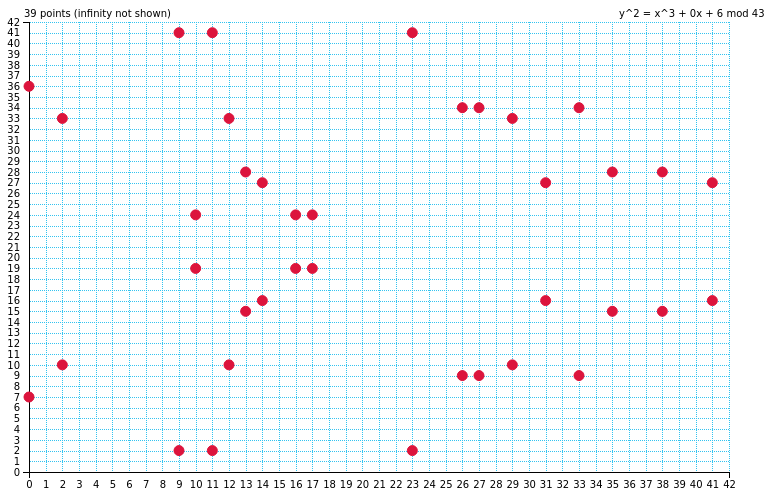
\includegraphics[scale=0.6]{figures/bls6-6.png}
As we can see our curve is somewhat nice, as it does not contain self inverse points that is points with $y=0$. It follows that the addition law can be optimized, since the branch for those cases can be eliminated. 

Note: Is there a way to printe the entire addition table from https://graui.de/code/elliptic2/ here? Would be nice to have but is a bit large.

Since the order of BLS6-6 is $39= 3\cdot 13$, we know that it has a "large" subgroup of order $13$ and small subgroup of order $3$. We can use XXX to find those groups. We have $BLS6-6(3)=\{\mathcal{O},(0,7),(0,36)\}$.

In addition we have the generator $g_{BLS6}:=(13,15)$ that generates
\begin{multline}
BLS6-6(13)=\\
\{(13,15) \rightarrow (33,34) \rightarrow  (38,15) \rightarrow  (35,28) \rightarrow (26,34) \rightarrow  (27,34) \rightarrow  \\ 
(27,9)  \rightarrow  (26,9) \rightarrow  (35,15) \rightarrow  (38,28) \rightarrow  (33,9) \rightarrow (13,28) \rightarrow  \mathcal{O}\}$$
\end{multline}

Computations "in the exponent": In cryptography and in particular in snarks a lot HAPPENS IN THE EXPONENT...

To use our example to explain what this means observe that from this representation, we can deduce a map from the scalar field $\F_{13}$ to $BLS6-6(13)$ with respect to our generator. WE have
$$
[\cdot]_{(13,15)}: \F_{13} \to BLS6-6(13)\;;\; x \mapsto [x](13,15)
$$

So for example we have $[1]_{(13,15)}= (13,15)$, $[7]_{(13,15)}= (27,9)$ and $[0]_{(13,15)}= \mathcal{O}$. In particular this map is a homomorphism of groups from the additive group $\F_{13}$ to $BLS6-6(13)$. This means in particular, the the additive neutral element from $\F_{13}$ is mapped to $\mathcal{O}$ and negatives are mapped to inverses. For example $[-2]_{(13,15)}= - [2]_{(13,15)}$, since
$[-2]_{(13,15)}= [11]_{(13,15)}= (33,9) = (33,-34) = -(33,34)=
- [2]_{(13,15)}$

The map also give a visualization of the ECDL problem in $BLS6-6(13)$, which is concerned with finding solutions $x\in \F_{13}$ for the equation 
$[x]_{(13,15)}= (x,y)$ for any $(x,y) \in BLS6-6(13)$. Of course ECDL is not hard in $BLS6-6(13)$, since we can deduce the solutions easily from XXX. For example the solution to $[x]_{(13,15)}= (35,15)$ is $x=9$, since $[9](13,15)=(35,15)$.

Since $[0]_{(13,15)}$ maps the group of cyclic integers modulo $13$ onto our group $BLS6-6(13)$, we can use this to write down the group law in the following way:
\begingroup
    \fontsize{5pt}{5pt}\selectfont
$$
\begin{array}{c|ccccccccccccc}
\cdot & \mathcal{O}  & (13,15) & (33,34) & (38,15) & (35,28) & (26,34) & (27,34) & (27,9) & (26,9) & (35,15) & (38,28) & (33,9) & (13,28)\\
\hline
\\
\mathcal{O} & \mathcal{O}  & (13,15) & (33,34) & (38,15) & (35,28) & (26,34) & (27,34) & (27,9) & (26,9) & (35,15) & (38,28) & (33,9) & (13,28)\\
\\
(13,15) & (13,15) & (33,34) & (38,15) & (35,28) & (26,34) & (27,34) & (27,9) & (26,9) & (35,15) & (38,28) & (33,9) & (13,28) & \mathcal{O}\\
\\
(33,34) & (33,34) & (38,15) & (35,28) & (26,34) & (27,34) & (27,9) & (26,9) & (35,15) & (38,28) & (33,9) & (13,28) & \mathcal{O} & (13,15)\\
\\
(38,15) & (38,15) & (35,28) & (26,34) & (27,34) & (27,9) & (26,9) & (35,15) & (38,28) & (33,9) & (13,28) & \mathcal{O} & (13,15) & (33,34)\\
\\
(35,28) & (35,28) & (26,34) & (27,34) & (27,9) & (26,9) & (35,15) & (38,28) & (33,9) & (13,28) & \mathcal{O} & (13,15) & (33,34) & (38,15)\\
\\
(26,34) & (26,34) & (27,34) & (27,9) & (26,9) & (35,15) & (38,28) & (33,9) & (13,28) & \mathcal{O} & (13,15) & (33,34) & (38,15) & (35,28)\\
\\
(27,34) & (27,34) & (27,9) & (26,9) & (35,15) & (38,28) & (33,9) & (13,28) & \mathcal{O} & (13,15) & (33,34) & (38,15) & (35,28) & (26,34)\\
\\
(27,9) & (27,9) & (26,9) & (35,15) & (38,28) & (33,9) & (13,28) & \mathcal{O} & (13,15) & (33,34) & (38,15) & (35,28) & (26,34) & (27,34)\\
\\
(26,9) & (26,9) & (35,15) & (38,28) & (33,9) & (13,28) & \mathcal{O} & (13,15) & (33,34) & (38,15) & (35,28) & (26,34) & (27,34) & (27,9)\\
\\
(35,15) & (35,15) & (38,28) & (33,9) & (13,28) & \mathcal{O} & (13,15) & (33,34) & (38,15) & (35,28) & (26,34) & (27,34) & (27,9) & (26,9)\\
\\
(38,28) & (38,28) & (33,9) & (13,28) & \mathcal{O} & (13,15) & (33,34) & (38,15) & (35,28) & (26,34) & (27,34) & (27,9) & (26,9) & (35,15)\\
\\
(33,9) & (33,9) & (13,28) & \mathcal{O} & (13,15) & (33,34) & (38,15) & (35,28) & (26,34) & (27,34) & (27,9) & (26,9) & (35,15) & (38,28)\\
\\
(13,28) & (13,28) & \mathcal{O} & (13,15) & (33,34) & (38,15) & (35,28) & (26,34) & (27,34) & (27,9) & (26,9) & (35,15) & (38,28) & (33,9)\\
\end{array}
$$
\endgroup


Cofactor clearing: 

Given an arbitrary point on the curve that is not in any of our two subgroups like $(2,33)$, we can project it on both subgroups $BLS6-6(3)$ and $BLS6-6(13)$ respectively, by \textit{multiplication with the cofactor}. Since $39 = 3 \cdot 13$, we have to multiply $(2,33)$ with $13$ to map it onto $BLS6-6(3)$ and we have to multiply $(2,33)$ with $3$ to map it onto $BLS6-6(13)$. Indeed we get $[13](2,33)= (0,36)$ which is an element of $BLS6-6(3)$ and $[3](2,33)= (35,15)$ which is an element of $BLS6-6(13)$

In what follows we want to compute type 2 pairings on our BLS6 curve. We therefore need to extract the subgroup $\mathbb{G}_1$ as well as $\mathbb{G}_2$ from the full $13$-torsion group. We already know from XXX that $\mathbb{G}_1$ is given by  
\begin{multline*}
\mathbb{G}_1=\{(13,15) \rightarrow (33,34) \rightarrow  (38,15) \rightarrow  (35,28) \rightarrow (26,34) \rightarrow  (27,34) \rightarrow  \\ 
(27,9)  \rightarrow  (26,9) \rightarrow  (35,15) \rightarrow  (38,28) \rightarrow  (33,9) \rightarrow (13,28) \rightarrow  \mathcal{O}\}$$
\end{multline*}

In type 2 pairings, the group $\mathbb{G}_2$ is defined by those elements $P$ of the full $13$-torsion group, that are mapped to $43\cdot P$ under the Frobenius endomorphism XXX. Since $BLS6/\F_{13^6}$ contains $6321251664$ elements, we can not simply loop through all elements, to find the full $13$-torsion group and extract all elements from $\mathbb{G}_2$. However we can derive the full $13$-torsion as the set of all $13$-division points and then extract $G_2$ from this
\begin{sagecommandline}
sage: F43 = GF(43)
sage: F43t.<t> = F43[]
sage: F43_6.<v> = GF(43^6, name='v', modulus=t^6+6) # t^6+6 irreducible
sage: BLS6 = EllipticCurve (F43_6,[0 ,6])
sage: INF = BLS6(0) # point at infinity
sage: for P in INF.division_points(13): # PI(P) == [q]P
....:     if P.order() == 13: # exclude point at infinity
....:         PiP = BLS6([a.frobenius() for a in P])
....:         qP = 43*P
....:         if PiP == qP:
....:             print(P.xy())
\end{sagecommandline}

Choose $g_2=(7v^2, 16v^3)$ as generator of $\mathbb{G}_2$, we get
\begin{multline*}
\mathbb{G}_2=\{
(7v^2, 16v^3) \to
(10v^2, 28v^3)\to
(42v^2, 16v^3)\to
(37v^2, 27v^3)\to\\
(16v^2, 28v^3)\to
(17v^2, 28v^3)\to
(17v^2, 15v^3)\to
(16v^2, 15v^3)\to\\
(37v^2, 16v^3)\to
(42v^2, 27v^3)\to
(10v^2, 15v^3)\to
(7v^2, 27v^3)\to
\mathcal{O}\}
\end{multline*}
e.g. $[3]g_2= (42v^2, 16v^3)$.

Having those groups we can do pairings. We choose the Weil pairing and invoke sagemath. For example the Weil pairing between our two generators is
$$
e(g_1,g_2)= 5v^5 + 16v^4 + 16v^3 + 15v^2 + 3v + 41
$$

\begin{sagecommandline}
sage: g1 = BLS6([13,15])
sage: g2 = BLS6([7*v^2, 16*v^3])
sage: g1.weil_pairing(g2,13)
\end{sagecommandline}

As we have seen, $\mathbb{G}_2$ needs quite a bit more storage space then $\mathbb{G}_1$, since elements in $\mathbb{G}_2$ are pairs of polynomials of degree $<6$ with coefficients in $\F_{43}$, while elements from $\mathbb{G}_1$ are just pairs of elements from $\F_{43}$. 

As we know from XXX it is possible to reduce the space needed to store $\mathbb{G}_2$ by using the concept of a twist. In our case $BLS6$ has embedding degree $6$ and the curve parameter $a$ in $y^2 = x^3 +ax + b$ is zero. We therefore know from XXX, that BLS6 has three different twist: A quadratic twist, a cubic twist and a sextic twist. We want to compute all of these twist:

The quadratic twisted BLS6-6 curve: Consider our BLS6-6 curve $BLS6-6/\F_{43^6}$. A quadratic twist is then another curve $BLS6-6_{2-twist}$ over $\F_{43^3}$ isomorphic to the original curve. We use XXX. The task is to find an $\omega\in \F_{43^6}$, such that $\omega^2 \in \F_{43^3}$. 
We choose $\omega = x^4 + 7x^3 + 9x^2 + 11x + 8$. Then we interpret $\delta = \omega^2 = 27x^2 + 17x + 35$ as an element from $\F_{43^3}$. So our twisted curve is
$y^2 = x^3+a\delta^2 x+b \delta^3 = x^3+6\cdot(27t^2+17t+35)$
so we get
$$
BLS6-6_{2-twist}/\F_{43^3}: y^2 = x^3+(10t^2+14t+15)
$$
\subsubsection{Baby JubJub}
% As we talk about R1CS already may write elliptic curves chapter after circuits/r1cs?
To give an understanding what the Baby-JubJub curve is, we want to parallel its development here to find a Baby-Jubjub like curve for pen and paper.

As with the original large Baby-JubJub curve we apply the method from
%https://www.hjp.at/doc/rfc/rfc7748.html#page_19 (Appendinx A)
to define a pen\& paper Baby-JubJub-like curve over the scalar field of the "large" BLS6 prime order subgroup, which is $\F_{13}$. 

Since $\Zmod{13}{4}=1$ we would go with A.1. As we will only find a few curves, we will tweak the algorithm and run
\begin{sagecommandline}
sage: F13 = GF(13) 
sage: for A in xrange(3, 13):
....:     if (A-2) % 4 != 0:
....:         continue
....:     try:
....:         E = EllipticCurve(F13, [0, A, 0, 1, 0]) # Montgomery form
....:         E
....:         E.order()
....:     except:               
....:         continue      
\end{sagecommandline}
So we get two curves in Montgomery form $y^2 = x^3 + 6*x^2 + x$ which has order $8$ and  $y^2 = x^3 + 10*x^2 + x$, which has order $16$. We could transform one of them into an Edwards curve, however   

So to find our Edwards curve, we will do exhaustive search rather 
\begin{sagecommandline}
sage: for d in F13:          
....:     j= ZZ(0)          
....:     for x in F13:
....:         for y in F13:                        
....:             if x^2+y^2 == 1+d*x^2*y^2:                           
....:                 j=j+1        
....:     print('d=',d)                
....:     print('order=',j)     
\end{sagecommandline}
and get $x^2+y^2= 1+7\cdot x^2y^2$ which has $20$ points. The associated Montgomery curve is then using XXX given by $8y^2 = x^3 + 6\cdot x^2 + x$.

So we define our Baby-JubJub Edwards curve to be
$$
EdBJJ/\F_{13}: x^2+y^2= 1+7\cdot x^2y^2
$$
with associated Montgomery form to be
$$
MBJJ/\F_{13}:8y^2 = x^3 + 6\cdot x^2 + x
$$
As $20=2\cdot 2\cdot 5$, we have a "large" prime order subgroup of order $5$ and a cofactor $4$. The group of rational points is
\begin{sagecommandline}
sage: for x in F13:                                   
....:     for y in F13:                                                                                
....:         if x^2+y^2 == F13(1)+F13(7)*x^2*y^2:                                                     
....:             print(x,y)
\end{sagecommandline}

$$
(0, 1),
(0, 12),
(1, 0),
(2, 4),
(2, 9),
(4, 2),
(4, 11),
(5, 6),
(5, 7),
(6, 5),
(6, 8),
(7, 5),
(7, 8),
(8, 6),
(8, 7),
(9, 2),
(9, 11),
(11, 4),
(11, 9),
(12, 0)
$$
with neutral element $(0,12)$

As expected we have a prime order subgroup of size $5$, which can be generated by $(11,9)$. We get $\{(11,9)\to (6,8)\to (7,8) \to (2,9) \to (0,1))\}$.

% rewrite into something nice
\begin{sagecommandline}
sage: def Edwards_add((x1,y1),(x2,y2),d):
....:     x3 = F13((F13(x1)*F13(y2)+F13(y1)*F13(x2))/((F13(1)+F13(d)*F13(x1)*F13
....: (x2)*F13(y1)*F13(y2))))
....:     y3 = F13((F13(y1)*F13(y2)-F13(x1)*F13(x2))/((F13(1)-F13(d)*F13(x1)*F13
....: (x2)*F13(y1)*F13(y2))))
....:     return (x3,y3)
\end{sagecommandline}

\paragraph{Hashing to the pairing groups}
We give various constructions to hash into $\mathbb{G}_1$ and $\mathbb{G}_2$. 

We start with hashing to the scalar field... TO APPEAR

Non of these techniques work for hashing into $\mathbb{G}_2$. We therefore implement Pederson's Hash for BLS6. 

We start with $\mathbb{G}_1$. Our goal is to define an $12$-bit bounded hash function
$$
H_{1}: \{0,1\}^{12} \to \mathbb{G}_1 
$$
Since $12= 3\cdot 4$ we "randomly" select $4$ uniformly distributed generators $\{(38, 15), (35,28), (27, 34), (38, 28)\}$ from $\mathbb{G}_1$ and use the pseudo-random function from XXX. 
For every genrator we therefore have to choose a set of $4$ randomly generated invertible elements from $\F_{13}$. We choose
$$
\begin{array}{lcl}
(38,15) &:& \{2,7,5,9\}\\
(35,28) &:& \{11,4,7,7\}\\
(27,34) &:& \{5,3,7,12\}\\
(38,28) &:& \{6,5,1,8\}
\end{array}
$$
So our hash function is computed like this:
\begin{multline*}
H_1(x_{11},x_1,\ldots, x_{0})=
[2\cdot 7^{x_{11}}\cdot 5^{x_{10}}\cdot 9^{x_9}](38,15)+
[11\cdot 4^{x_8}\cdot 7^{x_7}\cdot 7^{x_6}](35,28)+\\
[5\cdot 3^{x_5}\cdot 7^{x_4}\cdot 12^{x_3}](27,34) +
[6\cdot 5^{x_2}\cdot 1^{x_{1}}\cdot 8^{x_{0}}](38,28)
\end{multline*}
Note that $a^x=1$ whe $x=0$ and hence those terms can be omitted in the computation. 
In particular the hash of the $12$-bit zero string is given by 
\begin{multline*}WRONG-ORDERING-REDO
H_1(0)= [2](38,15)+[11](35,28)+[5](27,34)+[6](38,28)= \\
(27,34)+(26,34)+(35,28)+(26,9)= (33,9) + (13,28) = (38,28)
\end{multline*}
The hash of $011010101100$ is given by 
\begin{multline*}
H_1(011010101100)=WRONG-ORDERING-REDO\\
[2\cdot 7^{0}\cdot 5^{1}\cdot 9^{1}](38,15)+
[11\cdot 4^{0}\cdot 7^{1}\cdot 7^{0}](35,28)+
[5\cdot 3^{1}\cdot 7^{0}\cdot 12^{1}](27,34) +
[6\cdot 5^{1}\cdot 1^{0}\cdot 8^{0}](38,28)=\\
[2\cdot 5\cdot 9](38,15)+
[11\cdot 7](35,28)+
[5\cdot 3\cdot 12](27,34) +
[6\cdot 5](38,28)=\\
[12](38,15)+
[12](35,28)+
[11](27,34) +
[4](38,28)=\\ 
TO_APPEAR
\end{multline*}
We can use the same technique to define a $12$-bit bounded hash function in $\mathbb{G}_2$:  
$$
H_{2}: \{0,1\}^{12} \to \mathbb{G}_2 
$$
Again we "randomly" select $4$ uniformly distributed generators $\{(7v^2 , 16v^3 ), (42v^2 , 16v^3 ), (17v^2 , 15v^3 ), (10v^2 , 15v^3 )\}$ from $\mathbb{G}_2$ and use the pseudo-random function from XXX. For every genrator we therefore have to choose a set of $4$ randomly generated invertible elements from $\F_{13}$. We choose
$$
\begin{array}{lcl}
(7v^2 , 16v^3 ) &:& \{8,4,5,7\}\\
(42v^2 , 16v^3 ) &:& \{12,1,3,8\}\\
(17v^2 , 15v^3 ) &:& \{2,3,9,11\}\\
(10v^2 , 15v^3 ) &:& \{3,6,9,10\}
\end{array}
$$
So our hash function is computed like this:
\begin{multline*}
H_1(x_{11},x_{10},\ldots, x_{0})=
[8\cdot 4^{x_{11}}\cdot 5^{x_{10}}\cdot 7^{x_9}](7v^2 , 16v^3)+
[12\cdot 1^{x_8}\cdot 3^{x_7}\cdot 8^{x_6}](42v^2 , 16v^3 )+\\
[2\cdot 3^{x_5}\cdot 9^{x_4}\cdot 11^{x_3}](17v^2 , 15v^3 ) +
[3\cdot 6^{x_2}\cdot 9^{x_{1}}\cdot 10^{x_{0}}](10v^2 , 15v^3 )
\end{multline*}
We extend this to a hash function that maps unbounded bitstring to $\mathbb{G}_2$ by precomposing with an actual haah function like $MD5$ and feet the first 12 bits of its outcome into our previously defined hash function. 
$$
TinyMD5_{\mathbb{G}_2}: \{0,1\}^* \to \mathbb{G}_2
$$
with $TinyMD5_{\mathbb{G}_2}(s)= H_2(MD5(s)_0,\ldots MD5(s)_{11})$. For example, since 
$MD5("")= 0xd41d8cd98f00b204e9800998ecf8427e$ and the binary representation of the hexadecimal number $0x27e$ is $001001111110$ we compute $TinyMD5_{\mathbb{G}_2}$ of the empty string as
$TinyMD5_{\mathbb{G}_2}("")= H_2(MD5(s)_{11},\ldots MD5(s)_{0}) = H2(001001111110)=$

\subsubsection{Baby-JubJub-2}
To give an understanding what the Baby-JubJub curve is, we want to parallel its development here to find a Baby-Jubjub like curve for pen and paper.

The original Baby-JubJub is a twisted Edwards curve over $\F_{?}$ with $a=-1$ and $d=?.$

As with the original large Baby-JubJub curve we apply the method from
%https://www.hjp.at/doc/rfc/rfc7748.html#page_19 (Appendinx A)
to define a pen\& paper Baby-JubJub-like curve over the scalar field of the "large" BLS6 prime order subgroup, which is $\F_{13}$. 

Since $\Zmod{13}{4}=1$ we would go with A.1. As we will only find a few curves, we will tweak the algorithm and run
\begin{sagecommandline}
sage: F13 = GF(13) 
sage: for A in xrange(3, 13):
....:     if (A-2) % 4 != 0:
....:         continue
....:     try:
....:         E = EllipticCurve(F13, [0, A, 0, 1, 0]) # Montgomery form
....:         E
....:         E.order()
....:     except:               
....:         continue      
\end{sagecommandline}
So we get two curves in Montgomery form $y^2 = x^3 + 6*x^2 + x$ which has order $8$ and  $y^2 = x^3 + 10*x^2 + x$, which has order $16$. We could transform one of them into an Edwards curve, however   

So to find our Edwards curve, we will do exhaustive search rather 
\begin{sagecommandline}
sage: j = ZZ(0)
sage: for a in F13:
....:     for d in F13:
....:         j = 0
....:         for x in F13:
....:             for y in F13:
....:                 if a*x^2 + y^2 == 1+d*x^2*y^2:
....:                     j=j+1
....:         print('curve: a=',a,'d=',d,'order:',j)     
\end{sagecommandline}
We want to choose a curve that has a large prime order subgroup and a small cofactor. So we go
with $2x^2+y^2= 1+3\cdot x^2y^2$ which has order $14$. 


The associated Montgomery curve is then using XXX given by $9y^2 = x^3 +2x^2 + x$.

So we define our Baby-JubJub Edwards curve to be
$$
EdBJJ/\F_{13}: 2x^2+y^2= 1+3\cdot x^2y^2
$$
with associated Montgomery form to be
$$
MBJJ/\F_{13}:9y^2 = x^3 + 2x^2 + x
$$
As $14=2\cdot 7$, we have a "large" prime order subgroup of order $7$ and a cofactor $2$. The group of rational points is
\begin{sagecommandline}
sage: for x in F13:                                   
....:     for y in F13:                                                                                
....:         if F13(2)*x^2+y^2 == F13(1)+F13(11)*x^2*y^2:                                                     
....:             print(x,y)
\end{sagecommandline}

$$
(0, 1),
(0, 12),
(2, 4),
(2, 9),
(4, 5),
(4, 8),
(5, 2),
(5, 11),
(8, 2),
(8, 11),
(9, 5),
(9, 8),
(11, 4),
(11, 9)
$$
with neutral element $(0,1)$

As expected we have a prime order subgroup of size $5$, which can be generated by $(11,9)$. We get $\{(11,9)\to (6,8)\to (7,8) \to (2,9) \to (0,1))\}$.

% rewrite into something nice
\begin{sagecommandline}
sage: def Edwards_add((x1,y1),(x2,y2),a,d):
....:     x3 = F13((F13(x1)*F13(y2)+F13(y1)*F13(x2))/((F13(1)+F13(d)*F13(x1)*F13(x2)*F13(y1)*F13(y2))))
....:     y3 = F13((F13(y1)*F13(y2)-F13(a)*F13(x1)*F13(x2))/((F13(1)-F13(d)*F13(x1)*F13(x2)*F13(y1)*F13(y2))))
....:     return (x3,y3)
\end{sagecommandline}




\subsection{MNT4 MNT6 Cycles}
% https://eprint.iacr.org/2006/372.pdf theorem 5.2
\begin{theorem}
Let $q$ be a prime and $E/\F_q$ be an ordinary elliptic curve such that $r= |E(Fq)|$ is a prime greater than $3$.  
\begin{itemize}
\item $E$ has embedding  degree $k= 4$ if and only if there  exists $x\in \mathbb{Z}$ such  that $t=-x$ or $t=x+1$, and $q=x^2+x+1$.\item $E$ has  embedding  degree $k= 6$ if and only if there  exists $x\in \Z$ such that $t= 1\pm 2x$ and $q=4x^2+1$.
\item There is an elliptic curve $E/\F_q$ with embedding degree $6$, discriminant $D$, and $|E(Fq)| = r$ if and only if there is an elliptic curve $E'/\F_r$ with embedding degree $4$, discriminant $D$, and $|E'(\F_r)| =q$.
\end{itemize}
\end{theorem}

We can use this theorem to find an MNT6-MNT4 cycle over very small prime fields with characteristics $>3$: 
\paragraph{MNT4}
For our MNT4 curve, we can choose $x=2$. Then $q=7$ and if we choose $t= x+1 $ then $r = q + 1 - t = 7 + 1 -3 = 5$. Therefore our MNT4 curve is a curve $y^2=x^3+ax+b$ defined over $\F_7$ that consists of $5$ points. 

To construct the actual curve we could use the complex multiplication method again, but since the parameters $a$ and $b$ are from $\F_7$ there are only $48$ possibilities so we simply loop through all possible $a$'s and $b$'s and count the curve points until we find a curve that has $5$ rational points. We get
$$
y^2 = x^3 + 4x + 1
$$
defined over $\F_7$, with scalar field $\F_5$. Since $7= 2^2+2+1$, we know from theorem XXX, that this curve has embedding degree $4$ and hence qualifies as a pen\&{}paper pairing friendly elliptic curve. Since the curve's order is a prime and therefore has no non trivial factors, it has no non trivial subgroups. The curve has the following set of elements
$$MNT4=\{(0,1)\to (0,6)\to (4,2)\to (4,5) \to \mathcal{O}\}$$ 
\begin{sagecommandline}
sage: F7 = GF(7)
sage: MNT4 = EllipticCurve (F7,[4 ,1])
sage: [P.xy() for P in MNT4.points() if P.order() > 1]
\end{sagecommandline}
The multiplication table is
\begingroup
    \fontsize{10pt}{10pt}\selectfont
$$
\begin{array}{c|ccccc}
\cdot & \mathcal{O} & (0,1) & (4,5) & (4,2) & (0,6)\\
\hline
\\
\mathcal{O} & \mathcal{O} & (0,1) & (4,5) & (4,2) & (0,6)\\
\\
(0,1) & (0,1) & (4,5) & (4,2) & (0,6) & \mathcal{O}\\
\\
(4,5) & (4,5) & (4,2) & (0,6) & \mathcal{O} & (0,1)\\
\\
(4,2) & (4,2) & (0,6) & \mathcal{O} & (0,1) & (4,5)\\
\\
(0,6) & (0,6) & \mathcal{O} & (0,1) & (4,5) & (4,2)\\
\end{array}
$$
\endgroup
In what follows we choose our generator to be $g_{MNT4}=(0,1)$.

In what follows we want to compute type 2 pairings on our MNT4 curve. We therefore need to extract the subgroup $\mathbb{G}_1$ as well as $\mathbb{G}_2$ from the full $5$-torsion group. Since the order of MNT4 is a prime number, we already know from XXX that $\mathbb{G}_1$ is given by  
$$\mathbb{G}_1=\{(0,1)\to (0,6)\to (4,2)\to (4,5) \to \mathcal{O}\}$$ 

In type 2 pairings, the group $\mathbb{G}_2$ is defined by those elements $P$ of the full $5$-torsion group, that are mapped to $7\cdot P$ under the Frobenius endomorphism XXX. Since $MNT4/\F_{7^4}$ only contains $2475$ elements, we can  loop through all elements, to find the full $5$-torsion group and extract all elements from $\mathbb{G}_2$:
\begin{sagecommandline}
sage: F7t.<t> = F7[]
sage: F7_4.<u> = GF(7^4, name='u', modulus=t^4+t+1) # embedding degree is 4
sage: MNT4 = EllipticCurve (F7_4,[4 ,1])
sage: INF = MNT4(0) # point at infinity
sage: for P in INF.division_points(5): # PI(P) == [q]P
....:     if P.order() == 5: # exclude point at infinity
....:         PiP = MNT4([a.frobenius() for a in P])
....:         qP = 7*P
....:         if PiP == qP:
....:             print(P.xy())
\end{sagecommandline}

Choose $g_2=(2u^3 + 5u^2 + 4u + 2, 2u^3 + 3u + 5)$ as generator of $\mathbb{G}_2$, we get
\begin{multline*}
\mathbb{G}_2=\{ 
(2u^3 + 5u^2 + 4u + 2, 2u^3 + 3u + 5) \to
(5u^3 + 2u^2 + 3u + 6, 2u^2 + 3u) \to \\
(5u^3 + 2u^2 + 3u + 6, 5u^2 + 4u) \to
(2u^3 + 5u^2 + 4u + 2, 5u^3 + 4u + 2)\to
\mathcal{O}\}
\end{multline*}
e.g. $[3]g_2= (5u^3 + 2u^2 + 3u + 6, 5u^2 + 4u)$.

Having those groups we can do pairings. We choose the Weil pairing and invoke sagemath. For example the Weil pairing between our two generators is
$$
e(g_1,g_2)= 5u^3 + 2u^2 + 6u
$$
\begin{sagecommandline}
sage: g1 = MNT4([0,1])
sage: g2 = MNT4(2*u^3 + 5*u^2 + 4*u + 2, 2*u^3 + 3*u + 5)
sage: g1.weil_pairing(g2,5)
\end{sagecommandline}
The full pairing table can the be written as
\begingroup
    \fontsize{10pt}{10pt}\selectfont
    
% generate the table entries as:
% sage: for i in range(5):
% ....:     for j in range(5):
% ....:         p = (i*g1).weil_pairing((j*g2),5)
% ....:         print('e([',i,']g1,[',j,']g2=',p)         
    
    
$$
\begin{array}{c|lllll}
e(\cdot,\cdot)    & \mathcal{O} & g_1            & [2]g_1         & [3]g_1         & [4]g_1\\
\hline
\\
      \mathcal{O} & 1           & 1              & 1              & 1              & 1\\
\\
              g_2 & 1           & 5u^3+2u^2+6u   & 6u^3+5u^2+6    & 2u^3+u^2+2u+3  & u^3+6u^2+6u+4\\
\\
\left[2\right]g_2 & 1           & 6u^3+5u^2+6    & u^3+6u^2+6u+4  & 5u^3+2u^2+6u   & 2u^3+u^2+2u+3\\
\\
\left[3\right]g_2 & 1           & 2u^3+u^2+2u+3  & 5u^3+2u^2+6u   & u^3+6u^2+6u+4  & 6u^3+5u^2+6\\
\\
\left[4\right]g_2 & 1           & u^3+6u^2+6u+4  & 2u^3+u^2+2u+3  & 6u^3+5u^2+6    & 5u^3+2u^2+6u\\
\end{array}
$$
\endgroup

\paragraph{MNT6}
For our MNT6 curve, we can choose $x=1$. Then $q=5$ and if we choose $t= 1 + 2x $ then $r= q + 1 - t = 5 + 1 + 1 = 7$. Therefore our MNT6 curve is a curve $y^2=x^3+ax+b$ defined over $\F_5$ that consists of $7$ points. 

To construct the actual curve we could use the complex multiplication method again, but since the parameters $a$ and $b$ are from $\F_5$ there are only $24$ possibilities, we simply loop through all possible $a$'s and $b$'s and count the curve points until we find a curve that has $7$ rational points. We get
$$
y^2 = x^3 + 2x + 1
$$
defined over $\F_5$. Since $5= 4\cdot 1 + 1$, we know from theorem XXX, that this curve has embedding degree $6$ and hence qualifies as a pen\&{}paper pairing friendly elliptic curve. 

The curve has the following set of elements
$$MNT6=\{(1,2)\to (3,3)\to (0,1)\to (0,4)\to (3,2)\to (1,3)\to \mathcal{O}\}$$
The multiplication table is
\begingroup
    \fontsize{10pt}{10pt}\selectfont
$$
\begin{array}{c|ccccccc}
\cdot & \mathcal{O} & (1,2) & (3,3) & (0,1) & (0,4) & (3,2) & (1,3)\\
\hline
\\
\mathcal{O} & \mathcal{O} & (1,2) & (3,3) & (0,1) & (0,4) & (3,2) & (1,3)\\
\\
(1,2) & (1,2) & (3,3) & (0,1) & (0,4) & (3,2) & (1,3) & \mathcal{O}\\
\\
(3,3) & (3,3) & (0,1) & (0,4) & (3,2) & (1,3) & \mathcal{O} & (1,2)\\
\\
(0,1) & (0,1) & (0,4) & (3,2) & (1,3) & \mathcal{O} & (1,2) & (3,3)\\
\\
(0,4) & (0,4) & (3,2) & (1,3) & \mathcal{O} & (1,2) & (3,3) & (0,1)\\
\\
(3,2) & (3,2) & (1,3) & \mathcal{O} & (1,2) & (3,3) & (0,1) & (0,4)\\
\\
(1,3) & (1,3) & \mathcal{O} & (1,2) & (3,3) & (0,1) & (0,4) & (3,2)\\
\end{array}
$$
\endgroup

In what follows we choose our generator to be $g_{MNT6}=(1,2)$.

In what follows we want to compute type 2 pairings on our MNT6 curve. We therefore need to extract the subgroup $\mathbb{G}_1$ as well as $\mathbb{G}_2$ from the full $7$-torsion group. Since the order of MNT6 is a prime number, we already know from XXX that $\mathbb{G}_1$ is given by
$$\mathbb{G}_1=\{(1,2)\to (3,3)\to (0,1)\to (0,4)\to (3,2)\to (1,3)\to \mathcal{O}\}$$
In type 2 pairings, the group $\mathbb{G}_2$ is defined by those elements $P$ of the full $7$-torsion group, that are mapped to $5\cdot P$ under the Frobenius endomorphism XXX. Since $MNT6/\F_{5^6}$ contains $15680$ elements, we can still loop through all elements, to find the full $7$-torsion group and extract all elements from $\mathbb{G}_2$

\begin{sagecommandline}
sage: G.<x> = GF(5^6) # embedding degree is 6
sage: MNT6 = EllipticCurve (G,[2 ,1])
sage: INF = MNT6(0) # point at infinity
sage: for P in INF.division_points(7): # PI(P) == [q]P
....:     if P.order() == 7: # exclude point at infinity
....:         PiP = MNT6([a.frobenius() for a in P])
....:         qP = 5*P
....:         if PiP == qP:
....:             print(P.xy())
\end{sagecommandline}

\begin{multline*}
\mathbb{G}_2=\{ 
(x^3+2x^2+4x,x^5+2x^4+4x^3+3x^2+3)\to
(x^5+4x^4+2x^3+3x^2+x+2,3x^4+2x^3+x)\to\\
(4x^5+x^4+2x^3,3x^5+x^4+x^3+4x+4)\to
(4x^5+x^4+2x^3,2x^5+4x^4+4x^3+x+1) \to\\
(x^5+4x^4+2x^3+3x^2+x+2,2x^4+3x^3+4x)\to
(x^3+2x^2+4x,4x^5+3x^4+x^3+2x^2+2)\to
\mathcal{O}\}
\end{multline*}
We choose the generator $g_2 = (x^3+2x^2+4x,x^5+2x^4+4x^3+3x^2+3)$

\begin{remark}
Note however that our MNT6 curve discriminant $D=-16(4a^3 + 27 b^2)= -16(4\cdot 2^3 + 27\cdot 1^2)=-944$, while our MNT4 curve has discriminsnt XXX. Hence our example curves are not those guranteed by theorem XXX. Those curve are both given by $y^2= x^3 + 2x +1$ over $\F_5$ and $\F_7$, respectively. However as both curves have the same defining equation, we rather choose examples that are visually distinguishable by their defining equations.
\end{remark}

\subsection{Edwards curve cycles}
